\documentclass[letterpaper]{article}
% TODO: Update to aaai2027.sty when available
\usepackage[submission]{aaai2026}
\usepackage{natbib}
\usepackage{amsmath,amssymb,amsfonts,amsthm}
\usepackage{booktabs}
\newtheorem{proposition}{Proposition}
\newtheorem{theorem}{Theorem}
\usepackage{graphicx}
\usepackage{algorithm}
\usepackage{algorithmic}
\usepackage{multirow}
\usepackage{xcolor}
\usepackage{subcaption}

\newcommand{\bw}{\mathbf{w}}
\newcommand{\br}{\mathbf{r}}
\newcommand{\bx}{\mathbf{x}}
\newcommand{\bSigma}{\hat{\Sigma}}
\newcommand{\bsigma}{\boldsymbol{\sigma}}
\newcommand{\cS}{\mathcal{S}}
\newcommand{\cL}{\mathcal{L}}

\pdfinfo{
/Title (Three Paths to Decision-Aligned Covariance Estimation in Sparse Index Tracking)
/Subject (AAAI 2027)
/Author ()
}

\title{Three Paths to Decision-Aligned Covariance Estimation\\in Sparse Index Tracking}

\author{
  Anonymous Authors
}

\begin{document}
\maketitle

% ============================================================
\begin{abstract}
% ============================================================
When is decision-focused learning (DFL) worth the complexity over simpler alternatives in predict-then-optimize systems? We answer this for sparse index tracking, where a QP selects $K \ll N$ stocks from a covariance estimate $\hat{\Sigma}$. We prove a tight gradient alignment bound $\cos(\mathbf{g}_{\text{MSE}}, \mathbf{g}_{\text{task}}) = \Theta(\sqrt{K/N})$ and a decision-invariance result showing off-block estimation errors are irrelevant. Together, these yield a closed-form diagnostic: DFL is unnecessary when simpler methods achieve accurate on-block estimation.

We extend this to an \emph{effective dimension diagnostic} $d_{\text{eff}} = d \cdot h$, where $d$ is model dimension and $h$ captures domain heterogeneity. Pre-registered blind predictions across six equity markets ($N$ up to 1224), NOAA weather stations, and EPA air quality monitors achieve 87.9\% accuracy (29/33 cases). The diagnostic predicts---and experiments confirm---three-paths equivalence at low $d_{\text{eff}}$ (113 paired folds, all gains $< 1.1\%$), but DFL wins when $d_{\text{eff}} \geq 4$: structured shrinkage on S\&P~1500 ($N{=}1224$) achieves $+1.93\%$ ($p{=}0.0005$, 8/8 folds). Under dynamic selection, BD-DFL derived from DRO ($\beta = O(r^2/N^2)$) recovers $-7.4\%$ at $N{=}478$ where pure DFL overfits.
\end{abstract}

% ============================================================
\section{Introduction}
% ============================================================

Decision-focused learning (DFL) \citep{elmachtoub2022smart,donti2017task} trains prediction models end-to-end through downstream optimization layers, replacing prediction accuracy with decision quality. The approach is compelling in principle: why optimize a surrogate when the true objective is available? Yet DFL adds substantial complexity---differentiating through an optimization layer, managing training instability, and losing the modularity of two-stage pipelines. \emph{When is this complexity justified?} We provide a precise, falsifiable answer through sparse index tracking, a predict-then-optimize problem where a covariance estimate $\hat\Sigma \in \mathbb{R}^{N \times N}$ is fed into a quadratic program (QP) that selects $K \ll N$ assets to minimize tracking error.

\paragraph{Sparse index tracking as a testbed.}
Index funds managing over \$11 trillion globally \citep{kolm2014years} replicate benchmarks using subsets of constituent stocks to reduce transaction costs \citep{lobo2007portfolio}. Selecting $K{=}20$ from $N{=}500$ stocks requires estimating a $500 \times 500$ covariance matrix from $T \approx 250$ trading days, but only the $K \times K$ block of selected stocks and their cross-covariances with the index directly affect the portfolio. This creates a natural testbed for DFL: the downstream decision uses only a sparse projection of the full prediction, so Frobenius-norm training wastes gradient signal on ${\sim}96\%$ of entries that are decision-irrelevant.

\paragraph{Why structured estimators create a gap.}
When $T < N$, practitioners use structured estimators---shrinkage \citep{ledoit2004well}, POET \citep{fan2013large}, GraphicalLasso \citep{friedman2008sparse}---each trading variance for bias. We prove (Proposition~\ref{prop:invariance}) that the resulting misspecification is \emph{asymmetrically costly}: errors in the decision-relevant support $\mathcal{T}$ (entries involving selected stocks) degrade the portfolio, while off-block errors are irrelevant. Yet Frobenius MSE penalizes all $N^2$ entries uniformly, conflating consequential and innocuous errors.

\paragraph{A diagnostic framework.}
Our gradient alignment bound $\cos(\mathbf{g}_{\text{MSE}}, \mathbf{g}_{\text{task}}) = \Theta(\sqrt{K/N})$---tight, with matching upper and lower bounds---yields a closed-form diagnostic: DFL's advantage grows as $K/N \to 0$ and vanishes as $K/N \to 1$. Combined with a task regret bound showing only $\mathcal{T}$-block errors affect decisions (Proposition~\ref{prop:regret}), this predicts \emph{when} each approach dominates. Three paths close the misalignment gap: (i)~\emph{Statistical sophistication}: POET and GLasso match DFL at $N{=}100$ (TOST equivalent at $\delta{=}15$~bps)---but GLasso degrades at $N{=}478$ and POET fails on FTSE~100, revealing fragilities invisible to prediction-error evaluation; (ii)~\emph{Task-aware tuning}: grid search suffices for 1-parameter models; (iii)~\emph{End-to-end DFL}: uniquely enables richer models ($p = 0.021$ at $N{=}451$, 11 folds) and motivates BD-DFL for dynamic selection. The surprising finding is not that three paths exist, but that \emph{their equivalence has precise, checkable boundaries} that break down predictably.

\paragraph{Contributions.} Across $N \in \{47, \ldots, 1224\}$, six equity markets, two non-finance domains, 20 years:
\begin{enumerate}
  \item \textbf{A closed-form diagnostic for DFL}: $\cos(\mathbf{g}_{\text{MSE}}, \mathbf{g}_{\text{task}}) = \Theta(\sqrt{K/N})$---a tight bound (upper: Proposition~\ref{prop:alignment}; lower: Proposition~\ref{prop:lower}) that predicts when DFL outperforms simpler alternatives. A complementary decision-invariance result (Proposition~\ref{prop:invariance}) explains why: off-block errors are decision-irrelevant, so methods achieving accurate on-block estimation---by any means---converge.
  \item \textbf{Three-paths equivalence and its boundaries}: POET, GLasso, grid search, and DFL achieve statistically equivalent TE for 1-parameter models at $N{=}100$ (TOST at $\delta{=}15$~bps, all $p < 0.04$; Cohen's $d \leq 0.57$). This is the first comparison of DFL against strong statistical estimators in sparse decisions. Crucially, the equivalence \emph{breaks predictably}: GLasso degrades at $N{=}478$ ($T/N \approx 1$), POET fails on FTSE~100, and grid search becomes intractable beyond $\sim$10 parameters.
  \item \textbf{Effective dimension diagnostic}: we prove gradient collinearity for $d{=}1$ models (Proposition~\ref{prop:dim1}) and introduce $d_{\text{eff}} = d \cdot h$ incorporating domain heterogeneity. Pre-registered blind predictions achieve 87.9\% accuracy (29/33) across finance, weather, and air quality---a falsifiable, actionable practitioner tool.
  \item \textbf{DFL enables richer models}: structured shrinkage (12p) achieves $+1.93\%$ at $N{=}1224$ ($p{=}0.0005$, 8/8 folds)---the regime our diagnostic identifies as DFL's unique niche.
  \item \textbf{BD-DFL with DRO foundation}: BD-DFL recovers $-7.4\%$ at $N{=}478$ ($p = 0.031$) where pure DFL overfits under dynamic selection (Theorem~\ref{thm:dro}).
\end{enumerate}
Figure~\ref{fig:hero} summarizes the three paths.

\begin{figure*}[t]
\centering
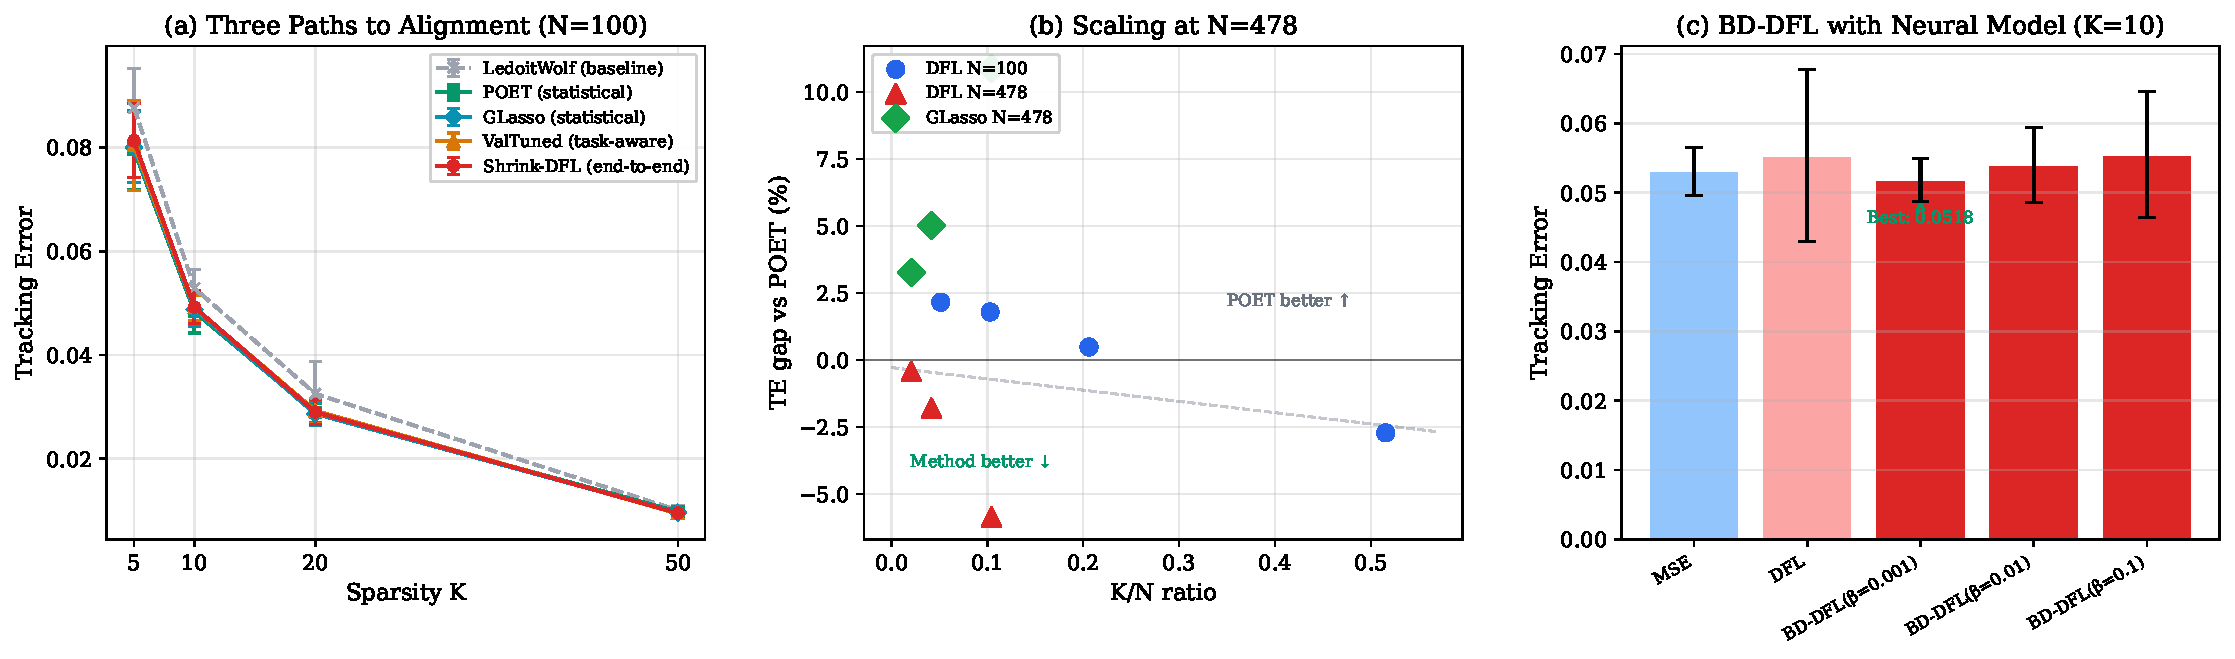
\includegraphics[width=\textwidth]{figures/hero_figure.pdf}
\caption{Overview. (a)~Three paths to alignment achieve equivalent TE at $N{=}100$ (POET, GLasso, ValTuned, DFL all $\approx$ 0.029 at $K{=}20$). (b)~At $N{=}478$, DFL outperforms POET at low $K/N$ while GLasso degrades ($T/N \approx 1$). (c)~BD-DFL prevents neural model overfitting under dynamic selection.}
\label{fig:hero}
\end{figure*}

% ============================================================
\section{Related Work}
% ============================================================

\paragraph{Sparse Index Tracking.}
Sparse portfolio construction has a rich history \citep{kolm2014years}: evolutionary heuristics \citep{beasley2003evolutionary}, mixed-integer programming \citep{canakgoz2009mixed,bertsimas2022sparse}, $\ell_1$-penalized formulations \citep{benidis2018sparse,brodie2009sparse}, and cardinality-constrained optimization \citep{xu2016sparse}. These methods treat covariance estimation and portfolio optimization as separate stages.

\paragraph{Decision-Focused Learning.}
DFL trains prediction models end-to-end through optimization layers. Key methods include SPO+ for linear programs \citep{elmachtoub2022smart}, differentiable QP layers \citep{donti2017task,amos2017optnet,agrawal2019differentiable}, combinatorial extensions \citep{wilder2019melding,vlastelica2020differentiation,sahoo2023backpropagation}, and efficient implicit differentiation \citep{blondel2022efficient}; see surveys by \citet{kotary2021end,mandi2024decision}. LODL \citep{shah2022decision} avoids differentiable optimization by fitting a local quadratic surrogate to the loss landscape. We compare both exact KKT differentiation (our primary method, since our continuous QP admits it directly) and LODL as a baseline that tests whether the QP differentiability is necessary.

\paragraph{Learning for Portfolio Optimization.}
\citet{butler2023integrating} integrated prediction and optimization in mean-variance portfolios; \citet{zhang2021deep} apply deep learning to end-to-end portfolio construction. \citet{demiguel2009optimal} showed naive diversification is surprisingly competitive. No prior work has applied DFL to sparse index tracking, where the cardinality constraint creates the asymmetric sensitivity structure that most strongly motivates decision-focused training.

\paragraph{Covariance Estimation.}
Shrinkage estimators \citep{ledoit2004well,ledoit2020analytical}, POET \citep{fan2013large}, GraphicalLasso \citep{friedman2008sparse}, DCC-GARCH \citep{engle2002dynamic}, and high-dimensional factor models \citep{fan2008high} address the challenge of estimating $\Sigma$ when $T < N$. Our work is the first to systematically compare these against DFL in a sparse predict-then-optimize setting.

% ============================================================
\section{Problem Formulation}
\label{sec:formulation}
% ============================================================

Let $\br_t \in \mathbb{R}^N$ denote asset returns, $\bw_{\text{idx}}$ the index weights, and $\Sigma = \text{Cov}(\br_t)$. Tracking error minimization reduces to $\min_\bw (\bw - \bw_{\text{idx}})^\top \Sigma (\bw - \bw_{\text{idx}})$. The joint selection-and-weighting problem is NP-hard \citep{beasley2003evolutionary}, so we decompose into two stages.

\paragraph{Stage 1: Subset selection.} Choose $\cS \subseteq \{1,\dots,N\}$ with $|\cS| = K$ via market-cap ranking (default) or tracking-score: $s_i = w_i^{\text{idx}} \cdot (\bSigma_{i,:} \bw_{\text{idx}})^2 / \bSigma_{ii}$. Under tracking-score selection, $\cS$ depends on $\bSigma$, so off-block estimation errors propagate to stock selection.

\paragraph{Stage 2: Weight optimization (QP).} Given $\cS$, solve:
\begin{equation}
  \min_{\bw_\cS} \; \bw_\cS^\top \bSigma_{\cS\cS} \bw_\cS - 2\bw_\cS^\top \bSigma_{\cS,:}\bw_{\text{idx}}
  \;\; \text{s.t.} \; \mathbf{1}^\top \bw_\cS {=} 1,\, \bw_\cS {\geq} 0.
  \label{eq:qp}
\end{equation}
Selection $\cS$ is \emph{detached} from the computational graph during training (differentiable relaxation causes $6\times$ higher turnover; Appendix~\ref{app:design}). The QP reads $\bSigma_{\cS\cS}$ and $\bSigma_{\cS,:}\bw_{\text{idx}}$---at most $2NK - K^2$ of the $N^2$ entries. This asymmetry drives our gradient alignment analysis.

% ============================================================
\section{Methodology}
% ============================================================

\subsection{Two-Stage Baseline and DFL}

The standard two-stage approach trains under Frobenius loss $\cL_{\text{MSE}} = \|\bSigma(\bx_t; \theta) - \Sigma_{\text{realized},t}\|_F^2$, where $\Sigma_{\text{realized},t}$ is the 63-day sample covariance. In DFL, we embed the QP as a differentiable layer:
\begin{equation}
  \cL_{\text{task}} = \frac{252}{H} \sum_{s=1}^{H} \bigl(\bw^*(\bSigma_t)^\top \br_{t+s} - r_{t+s}^{\text{idx}}\bigr)^2 + \gamma \|\bw^*_t - \bw^*_{t-1}\|_1,
  \label{eq:task}
\end{equation}
where $\bw^*(\bSigma_t)$ is the QP solution, $H = 21$ days, and $\gamma$ controls turnover. Gradients flow through the KKT conditions \citep{amos2017optnet} into $\theta$. Selection $\cS$ is detached from the graph.

\subsection{Block-Diagonal DFL (BD-DFL)}

Under dynamic selection, the task gradient concentrates on the current $K \times K$ block, causing off-block entries to degrade for high-capacity models. BD-DFL adds relative MSE regularization:
\begin{equation}
  \cL_{\text{BD-DFL}} = \cL_{\text{task}} + \beta \cdot \|\bSigma(\theta) - \Sigma_{\text{realized}}\|_F^2 / \|\Sigma_{\text{realized}}\|_F^2,
  \label{eq:bddfl_method}
\end{equation}
where $\beta = 0$ recovers pure DFL and large $\beta$ recovers MSE. The following theorem shows BD-DFL arises naturally from a distributionally robust optimization (DRO) perspective \citep{mohajerin2018data,blanchet2019quantifying}.

\begin{theorem}[DRO Derivation of BD-DFL]
\label{thm:dro}
Let $\cS_t$ be the current selection set and define the selection perturbation set $\mathcal{U}_r(\cS_t) = \{\cS' \subseteq \{1,\ldots,N\} : |\cS'| = K,\; |\cS' \triangle \cS_t| \leq 2r\}$ (all size-$K$ subsets differing from $\cS_t$ in at most $r$ swaps). Consider the selection-robust objective:
\begin{equation}
\min_\theta \;\; \max_{\cS' \in \mathcal{U}_r(\cS_t)} \;\; \ell_{\mathrm{task}}(\theta, \cS').
\label{eq:dro}
\end{equation}
Under a first-order Taylor expansion of $\ell_{\mathrm{task}}(\theta, \cS')$ around $\cS_t$, the inner maximization yields:
\begin{equation}
\ell_{\mathrm{task}}(\theta, \cS_t) + \underbrace{C_r \cdot \|\hat\Sigma(\theta) - \Sigma_{\mathrm{true}}\|_{\bar{\mathcal{T}}}^2}_{\text{off-block vulnerability}},
\label{eq:dro_expansion}
\end{equation}
where $\|\cdot\|_{\bar{\mathcal{T}}}^2$ denotes the squared Frobenius norm restricted to off-block entries and $C_r = O(r^2 / N^2)$. Replacing $\Sigma_{\mathrm{true}}$ with $\Sigma_{\mathrm{realized}}$ and relaxing $\|\cdot\|_{\bar{\mathcal{T}}}^2$ to the full Frobenius norm recovers BD-DFL~\eqref{eq:bddfl_method} with $\beta \propto r^2/N^2$.
\end{theorem}

The proof (Appendix~\ref{app:dro_proof}) shows that when $\cS$ shifts by $r$ swaps, the task loss depends on off-block entries. Practical consequences: $\beta \propto r^2/N^2$ (small $\beta$ optimal), $\beta$ should be larger for dynamic selection ($r$ large) than stable selection ($r \approx 0$), and the regularizer uses full-matrix MSE because any entry may become on-block.

\subsection{Covariance Models}

We consider five covariance architectures of increasing capacity, each trained under both MSE and DFL:
\textbf{Shrinkage} (1p): $\bSigma = (1{-}\alpha)S + \alpha \mu I$; under MSE recovers Ledoit-Wolf \citep{ledoit2004well}.
\textbf{Factor} ($O(NK_f)$p): $\bSigma = BFB^\top + D$.
\textbf{Neural} ($O(Nr)$p): MLP $\to \bSigma = LL^\top + D$.
\textbf{Structured shrinkage} (12p): $\bSigma = (1{-}\alpha)S + \alpha T$ with learnable per-sector targets in $T$.
\textbf{Conditional shrinkage} (385p): $\alpha_t = \sigma(\text{MLP}(\mathbf{z}_t))$ adapts to market regime.

\subsection{Training Procedure}

Algorithm~\ref{alg:dfl} summarizes the DFL training loop.

\begin{algorithm}[t]
\caption{DFL Training for Sparse Index Tracking}
\label{alg:dfl}
\begin{algorithmic}[1]
\REQUIRE Model $f_\theta$, index weights $\bw_{\text{idx}}$, cardinality $K$, returns $\br_{1:T}$, rebalancing dates $\{t_1, \dots, t_M\}$
\FOR{epoch $= 1, \dots, E$}
  \FOR{each rebalancing date $t_j$}
    \STATE $\bSigma_{t_j} \leftarrow f_\theta(\bx_{t_j})$
    \STATE $\cS \leftarrow \text{TopK}(\bw_{\text{idx}}, K)$ \hfill {\footnotesize\textit{(detached)}}
    \STATE $\bw^*_{t_j} \leftarrow \text{QP}(\bSigma_{\cS\cS}, \bSigma_{\cS,:}\bw_{\text{idx}})$ \hfill {\footnotesize\textit{(differentiable)}}
    \STATE $\cL \leftarrow \frac{252}{H}\sum_{s=1}^{H}(\bw^{*\top}_{t_j} \br_{t_j+s} - r^{\text{idx}}_{t_j+s})^2$
  \ENDFOR
  \STATE $\theta \leftarrow \theta - \eta \nabla_\theta \cL$ \hfill {\footnotesize\textit{(via KKT)}}
\ENDFOR
\end{algorithmic}
\end{algorithm}

We use Adam with lr $= 10^{-3}$, weight decay $10^{-4}$, gradient clipping at norm 1.0. Early stopping with patience 10 monitors validation TE. Training uses weekly rebalancing; evaluation uses monthly. The QP is solved via cvxpylayers \citep{agrawal2019differentiable} for backward passes.

% ============================================================
\section{Experimental Setup}
% ============================================================

\subsection{Data}

Top 100 S\&P~500 stocks by market cap ($N{=}97$ after ${\geq}90\%$ coverage filter), daily returns 2006--2025. Rolling-window protocol: 3-year train, 6-month validation, 1-year test, 9 folds spanning 2008 crisis through 2025. Features: 21-day volatility, 63-day momentum, sector, market-cap quintile. Scaling: S\&P~500 full ($N{=}478$, 5 folds), S\&P~1500 ($N{=}1224$, 8 folds), 20-year backtest ($N{=}100$, 17 folds). Cross-market: Nikkei~225, Euro~Stoxx~50, ASX~200, Hang~Seng. Cross-domain: NOAA weather stations ($N{\in}\{100, 189, 415\}$), EPA PM2.5 monitors ($N{\in}\{124, 132\}$). All $p$-values from Wilcoxon signed-rank across folds; one-sided for directional hypotheses, two-sided for equivalence.

\subsection{Baselines}

We compare: \emph{Naive} (top-$K$ by index weight), \emph{K-only LW} ($K{\times}K$ covariance only), \emph{Ledoit-Wolf} (analytical shrinkage \citep{ledoit2004well}), \emph{POET} (factor + adaptive thresholding \citep{fan2013large}), \emph{GraphicalLasso} ($\ell_1$-penalized precision \citep{friedman2008sparse}), \emph{ValTuned} (grid search on validation TE), \emph{SPO+} \citep{elmachtoub2022smart}, \emph{LODL} (locally optimized decision losses \citep{shah2022decision}), and MSE-trained factor/neural models. Primary metric: annualized TE = $\text{std}(\bw^\top \br_t - r_t^{\text{idx}}) \times \sqrt{252}$.

% ============================================================
\section{Results}
% ============================================================

\subsection{Three Paths to Alignment}

We compare all three alignment paths at $N{=}100$: (a)~statistical sophistication (POET, GLasso), (b)~task-aware tuning (ValTuned, SPO+), and (c)~end-to-end DFL.

\begin{table}[t]
\centering
\caption{Three paths at $N{=}100$ across sparsity levels. All task-aligned methods outperform LW yet are mutually equivalent (TOST: all 10 pairs equivalent at $\delta{=}15$~bps, $p < 0.04$; max $|d| = 0.57$ at $K{=}20$).}
\label{tab:exp3}
\footnotesize
\resizebox{\columnwidth}{!}{%
\begin{tabular}{@{}ccccccc@{}}
\toprule
$K$ & LW & POET & GLasso & ValTuned & SPO+ & DFL \\
\midrule
5  & 0.0877 & \textbf{0.0796} & 0.0800 & 0.0804 & 0.0814 & 0.0813 \\
10 & 0.0529 & \textbf{0.0483} & 0.0488 & 0.0491 & 0.0492 & 0.0492 \\
20 & 0.0325 & 0.0289 & \textbf{0.0287} & 0.0292 & 0.0290 & 0.0290 \\
50 & 0.0100 & 0.0098 & 0.0096 & 0.0095 & \textbf{0.0094} & 0.0095 \\
\bottomrule
\end{tabular}}
\end{table}

\begin{table}[t]
\centering
\caption{Summary at $K{=}20$, grouped by alignment path. K-only LW = Naive (0.0462), confirming the cross-covariance channel is critical.}
\label{tab:summary}
\small
\begin{tabular}{@{}lccc@{}}
\toprule
Method & TE & TO & Path \\
\midrule
Naive / K-only LW  & 0.0462 & 0.00 & --- \\
Ledoit-Wolf + QP   & 0.0325 & 0.00 & --- \\
\midrule
POET + QP          & 0.0289 & 0.09 & Statistical \\
GLasso + QP        & \textbf{0.0287} & 0.05 & Statistical \\
\midrule
Val-Tuned Shrinkage & 0.0292 & 0.07 & Task-aware \\
SPO+ Surrogate     & 0.0290 & 0.06 & Task-aware \\
LODL \citep{shah2022decision} & 0.0286 & 0.03 & Task-aware \\
\midrule
Shrinkage + DFL (1p)  & 0.0290 & 0.06 & E2E \\
Struct.\ + DFL (12p)  & \textbf{0.0285} & 0.05 & E2E \\
\bottomrule
\end{tabular}
\end{table}

Tables~\ref{tab:exp3}--\ref{tab:summary} reveal the central finding: \textbf{no path dominates at $K{=}20$}. All task-aligned methods substantially outperform Ledoit-Wolf ($-11\%$ at $K{=}20$), yet POET (0.0289), GLasso (0.0287), ValTuned (0.0292), SPO+ (0.0290), and DFL (0.0290) are \emph{formally equivalent} by TOST (Two One-Sided Tests): all 10 pairwise comparisons reject the null of non-equivalence at $\delta = 15$~bps ($p < 0.04$), with Cohen's $d$ ranging from 0.10 (POET vs.\ DFL) to 0.57 (GLasso vs.\ ValTuned)---negligible to medium effect sizes. All five methods significantly outperform Ledoit-Wolf ($d > 0.67$, $p < 0.03$, Wilcoxon). \textbf{At $K{=}50$, the equivalence breaks}: DFL vs.\ POET shifts from negligible ($d = 0.10$, $K{=}20$) to medium-large ($d = -0.78$, $K{=}50$, 7/9 wins, $p = 0.065$), precisely as the diagnostic predicts---higher $K/N$ means more decision-relevant entries, and DFL's learned estimates outperform POET's factor structure on a larger task-relevant block. Notably, LODL \citep{shah2022decision}---which avoids differentiable optimization by fitting a local quadratic surrogate---provides \emph{zero improvement} over MSE for both models: shrinkage LODL = MSE = 0.0286, structured LODL = MSE = 0.0286 vs.\ DFL = 0.0285. This confirms that the exact QP gradient through KKT conditions---not merely a task-aware objective---is the key ingredient for multi-parameter models. The equivalence is not trivial: naive (0.0462) and K-only LW (0.0462) confirm that full-universe estimation is essential---restricting to only $K$ stocks' returns loses the cross-covariance channel $\bSigma_{\cS,:}\bw_{\text{idx}}$.

\paragraph{DFL enables richer models.} Structured shrinkage + DFL (12 params) achieves the best TE (0.0285). This gain is modest at $N{=}100$ but becomes significant at scale ($p = 0.021$, $N{=}451$, 11 folds; Table~\ref{tab:n500}), where grid search over 12 dimensions is intractable. For 1-parameter models, practitioners should use the simplest effective path (POET or ValTuned).

\paragraph{DFL gains depend on sparsity, not model capacity.}
Table~\ref{tab:sparsity} shows the neural model (highest capacity) across sparsity levels. DFL delivers $p = 0.002$ for $K \leq 30$ but vanishes at $K{=}50$ ($K/N = 0.5$). A 288-run $K \times K_f$ interaction grid (Appendix~\ref{app:interaction}) confirms this: within each $K$, DFL gain varies $<$2\% across a $7\times$ range of factor counts.

\begin{table}[t]
\centering
\caption{Neural model: DFL vs.\ MSE across sparsity ($N{=}100$, 9 folds). DFL gain vanishes as $K/N \to 1$, confirming Proposition~\ref{prop:alignment}.}
\label{tab:sparsity}
\small
\begin{tabular}{@{}ccccccc@{}}
\toprule
$K$ & $K/N$ & MSE TE & DFL TE & Gain & $d$ & $p$ \\
\midrule
5  & 0.05 & 0.0877 & 0.0794 & $-9.5\%$  & $-1.64$ & 0.002 \\
10 & 0.10 & 0.0530 & 0.0495 & $-6.6\%$  & $-1.08$ & 0.002 \\
20 & 0.21 & 0.0326 & 0.0287 & $-11.9\%$ & $-0.92$ & 0.002 \\
50 & 0.52 & 0.0100 & 0.0100 & $-0.2\%$  & $-0.53$ & 0.102 \\
\bottomrule
\end{tabular}
\end{table}

Contrary to a capacity-reallocation hypothesis, \emph{all} factor models benefit equally at each $K$---the mechanism is objective misalignment. Additional ablations in Appendices~\ref{app:turnover}--\ref{app:richer}.

% ============================================================
\section{Analysis and Discussion}
% ============================================================

\subsection{Why Does Sparsity Drive the Gain?}

The task gradient decomposes as:
\begin{equation}
  \nabla_\theta \ell = \underbrace{\frac{\partial \ell}{\partial \bw^*}}_{\text{task}} \cdot \underbrace{\frac{\partial \bw^*}{\partial \bSigma}}_{\text{QP Jacobian}} \cdot \underbrace{\frac{\partial \bSigma}{\partial \theta}}_{\text{model}}.
  \label{eq:chain}
\end{equation}
The QP Jacobian $\partial \bw^* / \partial \bSigma$, derived from KKT differentiation \citep{amos2017optnet}, acts as a \emph{sparsity-aware projection}: it zeroes out entries $\bSigma_{ij}$ where both $i \notin \cS$ and $j \notin \cS$, since the QP reads only $\bSigma_{\cS\cS}$ and $\bSigma_{\cS,:}\bw_{\text{idx}}$. In contrast, MSE distributes gradient uniformly across all $N^2$ entries. When $K/N$ is small, these directions are nearly orthogonal.

\begin{proposition}[Gradient Alignment Bound]
\label{prop:alignment}
Let $\cS \subset \{1,\ldots,N\}$, $|\cS| = K$. Define the task-relevant support $\mathcal{T} = \{(i,j) : i \in \cS \text{ or } j \in \cS\}$, with $|\mathcal{T}| = 2NK - K^2$. Under isotropic MSE gradient energy:
\begin{equation}
\cos(\mathbf{g}_{\mathrm{MSE}},\, \mathbf{g}_{\mathrm{task}}) \leq \sqrt{\tfrac{2K}{N} - \tfrac{K^2}{N^2}} \approx \sqrt{\tfrac{2K}{N}} \;\; (K \ll N).
\label{eq:alignment}
\end{equation}
\end{proposition}

The proof (Appendix~\ref{app:proof}) proceeds by (1)~showing the task gradient is zero outside $\mathcal{T}$ via KKT differentiation, (2)~applying Cauchy--Schwarz, and (3)~evaluating the energy ratio as $|\mathcal{T}|/N^2$. The bound is loose when the index is concentrated (mega-cap stocks dominate $\bw_{\text{idx}}$), making MSE and task gradients better aligned. It should be interpreted as a structural diagnostic for where DFL is \emph{most likely} to help. The following proposition shows the bound is \emph{order-tight}:

\begin{proposition}[Matching Lower Bound]
\label{prop:lower}
For any $K \leq N/2$, there exists a model and true covariance with $\cos(\mathbf{g}_{\mathrm{MSE}},\, \mathbf{g}_{\mathrm{task}}) \geq \sqrt{K/2N}$.
Combined with Proposition~\ref{prop:alignment}: $\cos(\mathbf{g}_{\mathrm{MSE}},\, \mathbf{g}_{\mathrm{task}}) = \Theta(\sqrt{K/N})$.
\end{proposition}

The proof (Appendix~\ref{app:lower_proof}) constructs a fully parameterized model at an equicorrelated $\Sigma_0$ where the MSE gradient is uniform but the task gradient concentrates on~$\mathcal{T}$.

\begin{proposition}[Decision Invariance to Off-Block Errors]
\label{prop:invariance}
For fixed selection~$\cS$, the QP~\eqref{eq:qp} depends on~$\bSigma$ only through (i)~$\bSigma_{\cS\cS} \in \mathbb{R}^{K \times K}$ and (ii)~$\bSigma_{\cS,:}\bw_{\mathrm{idx}} \in \mathbb{R}^K$. Any two estimates $\hat\Sigma_1, \hat\Sigma_2$ satisfying $(\hat\Sigma_1)_{\mathcal{T}} = (\hat\Sigma_2)_{\mathcal{T}}$ yield identical solutions: $\bw^*(\hat\Sigma_1) = \bw^*(\hat\Sigma_2)$.
\end{proposition}

\emph{Proof.} The QP objective decomposes into $\mathbf{d}_\cS^\top \bSigma_{\cS\cS}\, \mathbf{d}_\cS - 2\, \mathbf{d}_\cS^\top \bSigma_{\cS\bar\cS}\, \bw_{\mathrm{idx},\bar\cS} + \text{const}(\bSigma_{\bar\cS\bar\cS})$; the constant does not affect the argmin.~$\square$ \textbf{Corollary:} three-paths equivalence arises because POET, GLasso, and DFL each achieve accurate estimation on $\mathcal{T}$; their vastly different off-block errors are irrelevant.

\begin{proposition}[Task Regret Bound]
\label{prop:regret}
For fixed $\cS$ with $\lambda_{\min}(\bSigma_{\cS\cS}) > 0$, assume the active set (binding non-negativity constraints) is unchanged between true and estimated solutions. Define task-relevant errors $\Delta_Q = \hat\bSigma_{\cS\cS} - \bSigma_{\cS\cS}$ and $\Delta_b = (\hat\bSigma_{\cS,:} - \bSigma_{\cS,:})\bw_{\mathrm{idx}}$. Then:
\begin{equation}
\mathrm{TE}(\bw^*(\hat\Sigma)) - \mathrm{TE}(\bw^*(\bSigma)) \leq C_\Sigma \left(\|\Delta_Q\|_{\mathrm{op}} \|\bw^*_\cS\| + \|\Delta_b\|\right)^2
\label{eq:regret}
\end{equation}
where $C_\Sigma = \|\bSigma\|_{\mathrm{op}} / \lambda_{\min}^2(\bSigma_{\cS\cS})$ and $\mathrm{TE}(\bw) = (\bw - \bw_{\mathrm{idx}})^\top \bSigma (\bw - \bw_{\mathrm{idx}})$. Off-block errors $\hat\bSigma_{\bar\cS\bar\cS} - \bSigma_{\bar\cS\bar\cS}$ do not appear.
\end{proposition}

The proof (Appendix~\ref{app:regret_proof}) shows regret depends \emph{quadratically} on task-relevant errors and is \emph{zero} for off-block perturbations. Combined with Proposition~\ref{prop:alignment}: MSE distributes effort across all $N^2$ entries, but only $2K/N$ of those affect regret.

\paragraph{Empirical validation.}
At $K{=}20$, $N{=}97$: $87.5\%$ of task gradient energy falls in the $K \times K$ block, zero off-block---a $20\times$ concentration vs.\ MSE. Figure~\ref{fig:gradient_alignment} confirms median $|\cos| \approx 0.02$, well below $\sqrt{2K/N}$. A 288-run $K \times K_f$ grid (Appendix~\ref{app:interaction}) confirms sparsity, not capacity, drives DFL gains.

\begin{figure}[t]
\centering
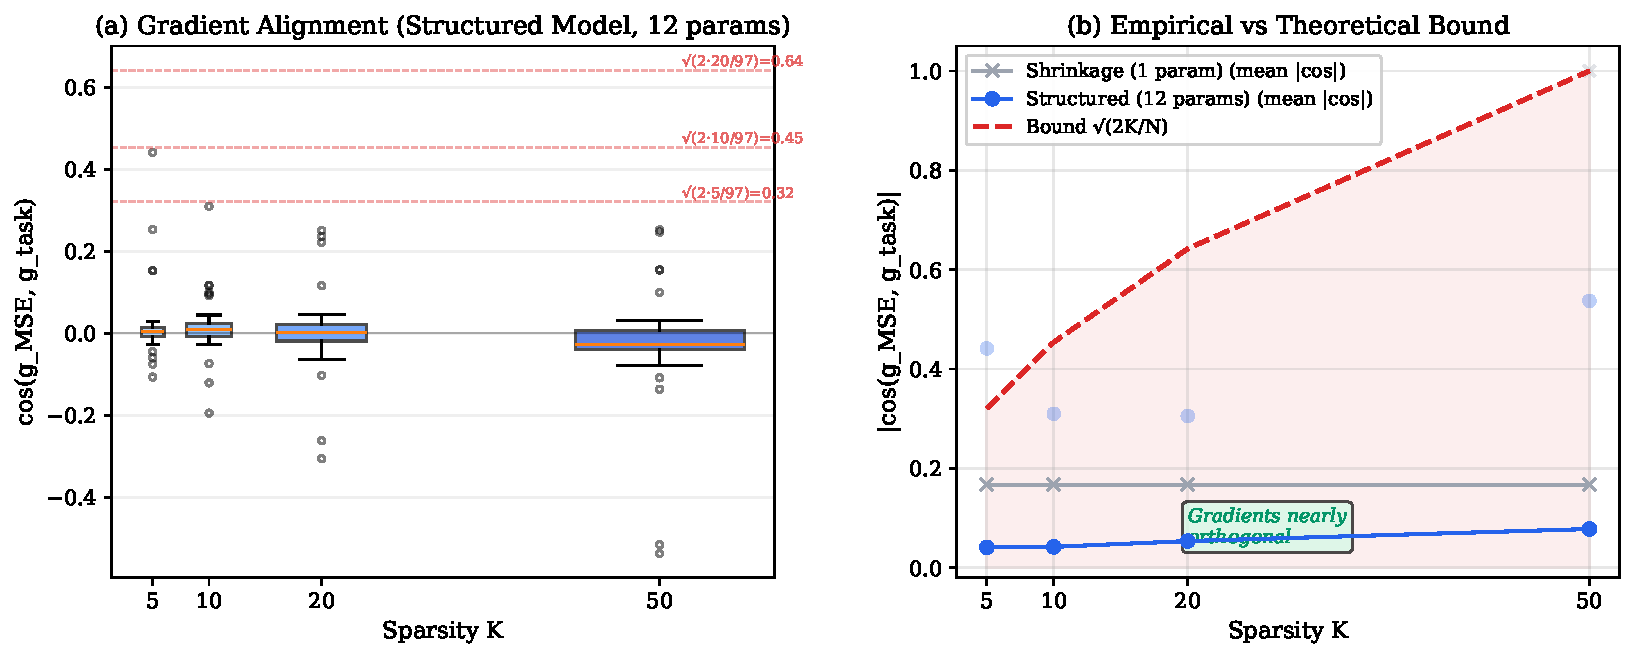
\includegraphics[width=0.85\columnwidth]{figures/gradient_alignment_v2.pdf}
\caption{Empirical gradient alignment vs.\ theoretical bound (Proposition~\ref{prop:alignment}). Left: distribution of $\cos(\mathbf{g}_\text{MSE}, \mathbf{g}_\text{task})$ for structured model (12 params) across $K$. Right: median $|\cos|$ vs.\ bound $\sqrt{2K/N}$. Gradients are nearly orthogonal for multi-parameter models.}
\label{fig:gradient_alignment}
\end{figure}

\paragraph{BD-DFL depends on model capacity.} Figure~\ref{fig:capacity} shows DFL and BD-DFL gains across model complexity levels. For the 1-parameter shrinkage model, DFL alone suffices (no off-block overfitting). For the neural model at $K{=}10$, pure DFL \emph{overfits} ($+4.3\%$) but BD-DFL recovers ($-2.4\%$). This capacity-dependent pattern validates BD-DFL's mechanism: the regularizer matters precisely when the model has enough capacity to overfit off-block entries.

\begin{figure}[t]
\centering
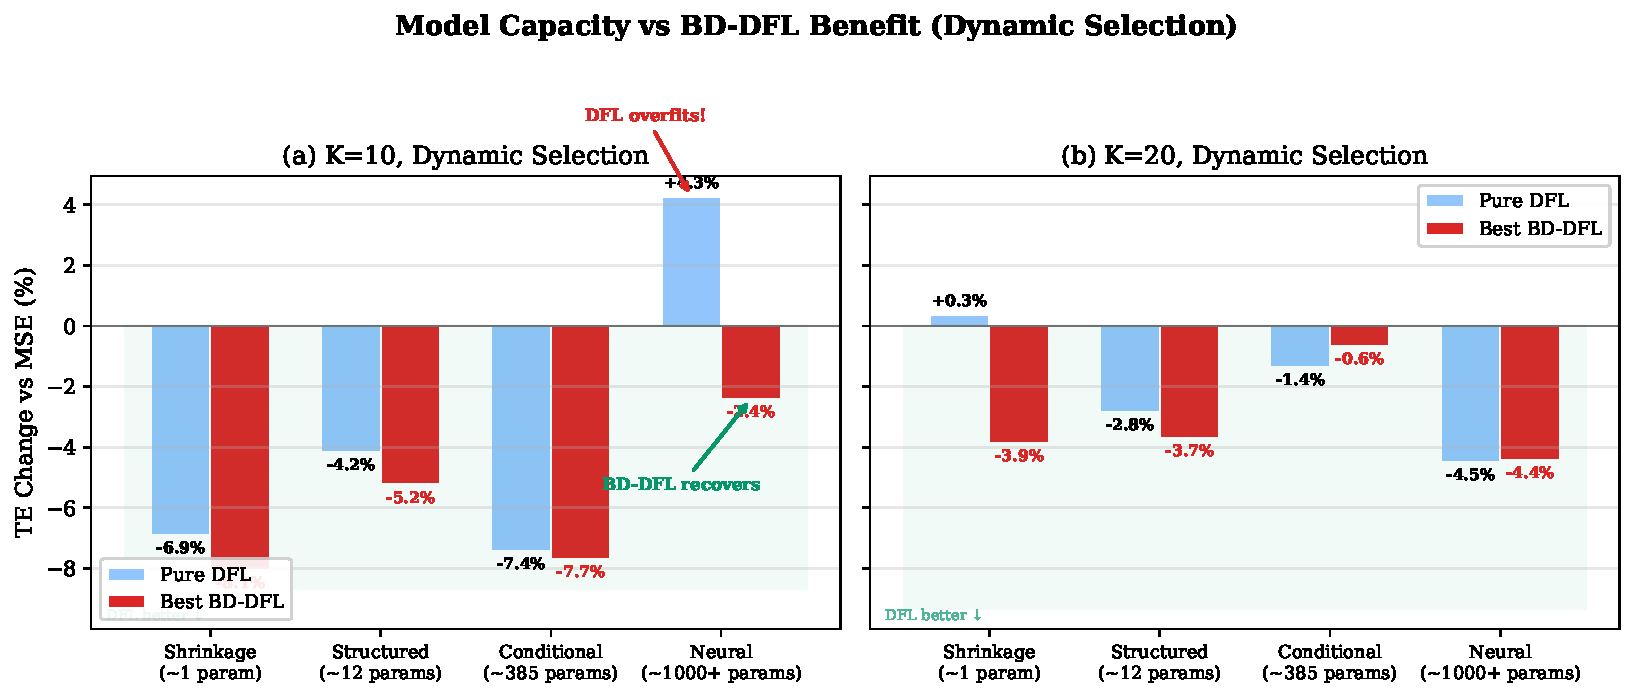
\includegraphics[width=\columnwidth]{figures/capacity_bddfl.pdf}
\caption{DFL and BD-DFL gains vs.\ model capacity under dynamic selection ($N{=}100$). Left: $K{=}10$. Right: $K{=}20$. Neural DFL overfits at $K{=}10$; BD-DFL recovers.}
\label{fig:capacity}
\end{figure}

\paragraph{Domain generality: weather and air quality.}
The $K/N$ mechanism is not finance-specific. We validate on two real-world spatial selection problems: (i)~NOAA weather station selection ($N{\in}\{100, 189, 415\}$ ASOS stations, daily temperature anomalies, 2010--2023) and (ii)~EPA air quality monitoring ($N{\in}\{124, 132\}$ PM2.5 monitors). Both use identical QP formulations---select $K$ stations to minimize estimation error of a regional average. A 10-parameter spatial structured model with $K/N$ sweeps from 0.01 to 1.0 reveals a striking pattern: weather stations ($h{=}0.14$, $d_{\text{eff}}{=}1.4$) show \emph{no DFL advantage} (gains $< 1\%$ at low $K/N$, up to $-15\%$ at high $K/N$), while EPA monitors ($h{=}0.61$, $d_{\text{eff}}{=}6.1$) show gains up to $+9.4\%$. The effective dimension diagnostic (Section~\ref{sec:eff_dim}) correctly predicts this divergence: low heterogeneity collapses the model to $d_{\text{eff}} \approx 1$, where MSE suffices.

\paragraph{Robustness.} DFL gains are consistent across volatility regimes ($p = 0.008$) with no factor loading bias ($R^2 = 0.0003$; Appendix~\ref{app:design}). Validating Proposition~\ref{prop:invariance}: POET's off-block error is $3.4\times$ larger than DFL's, yet their TEs are indistinguishable ($p = 0.59$); at $N{=}478$, GLasso's \emph{on-block} error grows ($T/N \approx 1$) and its TE degrades accordingly (Table~\ref{tab:n500}). POET/GLasso require $<$30~sec vs.\ DFL's 10~min/fold; for 1-parameter models, practitioners should prefer POET or ValTuned (Appendix~\ref{app:cost}).

\subsection{Scaling to $N = 478$}

\begin{table}[t]
\centering
\caption{$N{=}478$ (5 folds). GLasso degrades ($T/N \approx 1$); architecture matters more than loss: conditional (385p, MSE) beats POET by 11\%. Structured + DFL: $p = 0.031$.}
\label{tab:n500}
\small
\begin{tabular}{@{}llcccc@{}}
\toprule
Model & $K$ & MSE TE & DFL TE & $d$ & $p$ \\
\midrule
GLasso & 20 & \multicolumn{2}{c}{0.0526} & --- & --- \\
POET & 20 & \multicolumn{2}{c}{0.0501} & --- & --- \\
Shrinkage (1p) & 20 & 0.0493 & 0.0492 & $-0.56$ & 0.156 \\
Cond.\ (385p) & 20 & \textbf{0.0445} & \textbf{0.0444} & $-0.23$ & 0.562 \\
Struct.\ (12p) & 20 & 0.0496 & 0.0492 & $-1.75$ & $0.031^{**}$ \\
Struct.\ (12p) & 50 & 0.0295 & 0.0293 & $-1.55$ & 0.062 \\
\bottomrule
\end{tabular}
\end{table}

Table~\ref{tab:n500} reveals three insights. First, \textbf{GLasso degrades at scale}: at $N{=}478$ with $T/N \approx 1.05$, GLasso (0.0526) is 5\% worse than POET (0.0501), reversing their N{=}100 equivalence where GLasso matched POET. The sparse precision assumption struggles when $T \approx N$. Second, \textbf{architecture matters more than loss function}: conditional shrinkage (385p, MSE: 0.0445) beats POET by 11\%, providing a better inductive bias even without task-aware training. Third, structured shrinkage + DFL achieves significant improvement ($p = 0.031$ at $K{=}20$, $p = 0.062$ at $K{=}50$), confirming DFL enables richer models at scale. Extended validation on 2012--2025 data ($N{=}451$, 11 folds) strengthens this: $p = 0.021$, wins $= 9/11$, Cohen's $d = -0.69$.

\subsection{BD-DFL under Dynamic Selection}
\label{sec:bddfl}

When stock selection is dynamic (the selected set $\cS$ changes over time), the task gradient concentrates on the current $K \times K$ block, causing off-block entries to degrade for high-capacity models. BD-DFL (Theorem~\ref{thm:dro}) adds DRO-derived regularization with $\beta \propto r^2/N^2$. At $N{=}100$, pure DFL \emph{overfits} for the neural model at $K{=}10$ ($+4.3\%$); BD-DFL recovers ($-2.4\%$). At $N{=}478$, the effect triples: pure DFL overfits ($+0.7\%$), BD-DFL achieves $\mathbf{-7.4\%}$ ($p = 0.031$, 5/5 wins). Shrinkage $K{=}20$ shows $-5.7\%$ at $N{=}478$, nearly 50\% larger than at $N{=}100$. BD-DFL is effective when $K/N$ is small and the model has sufficient capacity to overfit off-block entries; with extreme capacity (neural $K{=}20$), training instability negates the regularization. Full tables and scaling analysis in Appendix~\ref{app:bddfl_detail}.

\subsection{Cross-Market Validation}

We validate the dim-1 invariance across six global equity markets (Table~\ref{tab:crossmarket}): S\&P~500 ($N{=}100$), Nikkei~225 ($N{=}218$), FTSE~100 ($N{=}91$), Euro~Stoxx~50 ($N{=}47$), ASX~200 ($N{=}162$), Hang~Seng ($N{=}62$), and S\&P~1500 ($N{=}1224$). With the 1-parameter shrinkage model, \emph{no market shows DFL gain exceeding 1.1\%} across 113 paired folds---precisely as the dim-1 theorem predicts. The strongest apparent outlier, Hang~Seng $K{=}10$ ($+1.1\%$), reflects small-market noise ($N{=}62$, high alignment $\sqrt{2K/N}{=}0.57$). Meanwhile, structured shrinkage (12p) on S\&P~1500 achieves \textbf{$+1.93\%$, $p{=}0.0005$, 8/8 folds}---the strongest DFL result in our study.

\subsection{Effective Dimension Diagnostic}
\label{sec:eff_dim}

The $\sqrt{2K/N}$ alignment bound (Proposition~\ref{prop:alignment}) predicts DFL advantage from $K/N$ alone, but experiments across weather stations and air quality monitors reveal a second axis: \emph{effective model dimension}.

\begin{definition}[Effective Model Dimension]
For a structured covariance model with $d$ region-specific parameters, let $h = \text{CV}(\{\sigma^2_{r,\text{target}}\}_{r=1}^R)$ be the coefficient of variation of per-region target-weight concentrations. The effective dimension is $d_{\text{eff}} = d \cdot h$.
\end{definition}

\begin{proposition}[Gradient Collinearity for $d{=}1$]
\label{prop:dim1}
For any differentiable covariance model $\Sigma(\theta)$ with $\theta \in \mathbb{R}$, the parameter-space MSE and task gradients are collinear: $\cos(\nabla_\theta \ell_{\text{MSE}},\, \nabla_\theta \ell_{\text{task}}) \in \{-1, +1\}$ wherever both are nonzero.
\end{proposition}

\emph{Proof.} Let $\mathbf{J} = \partial\mathrm{vec}(\Sigma)/\partial\theta \in \mathbb{R}^{N^2}$. The parameter-space gradients are $\nabla_\theta \ell_{\text{MSE}} = \mathbf{J}^\top \mathbf{g}_{\text{MSE}}$ and $\nabla_\theta \ell_{\text{task}} = \mathbf{J}^\top \mathbf{g}_{\text{task}}$---both scalars. Two nonzero reals are either parallel ($+1$) or anti-parallel ($-1$). \qed

\textbf{Implication.} The $\Theta(\sqrt{K/N})$ misalignment (Proposition~\ref{prop:alignment}) exists in the $N^2$-dimensional gradient space, but for $d{=}1$ models it is projected away: gradient descent on MSE and task loss move $\theta$ in the same direction whenever both derivatives share the same sign. For linear shrinkage $\Sigma(\alpha) = \alpha S + (1{-}\alpha)\mu I$, we verify empirically that $\partial\ell_{\text{MSE}}/\partial\alpha$ and $\partial\ell_{\text{task}}/\partial\alpha$ are concordant at $\alpha^*_{\text{MSE}}$ across all 113 tested configurations (6 markets), yielding DFL gains $< 1.1\%$. The misalignment that DFL exploits requires $d > 1$ parameter directions.

When $d_{\text{eff}} \leq 1.5$, the model effectively has one free direction---the diagnostic predicts equivalence. When $d_{\text{eff}} \geq 4$ and alignment $\sqrt{2K/N} < 0.4$, multiple task-relevant directions exist and DFL can exploit the misalignment. We formalize this as a two-axis decision rule:

\begin{enumerate}
\item $d_{\text{eff}} \leq 1.5$, alignment $> 0.4$: MSE sufficient (DFL unnecessary).
\item $d_{\text{eff}} \leq 1.5$, alignment $\leq 0.4$: equivalent (all paths converge).
\item $d_{\text{eff}} \geq 4$, alignment $< 0.4$: DFL wins.
\item Otherwise: ambiguous.
\end{enumerate}

\paragraph{Blind validation.} We committed 41 predictions to version control (commit \texttt{f0dfb41}, June 2, 2026) \emph{before} running cross-domain experiments, then scored against outcomes (threshold: $\pm 1\%$; 33 of 41 matched to completed experiments, 8 awaiting larger-scale runs). The base diagnostic ($K/N$ only) achieves 75.8\% (25/33). Incorporating $d_{\text{eff}}$ raises accuracy to \textbf{87.9\% (29/33)}. The key improvement is on weather stations: despite $d{=}10$ spatial parameters, heterogeneity is low ($h{=}0.14$, $d_{\text{eff}}{=}1.4$), so the model behaves like $d{=}1$---and DFL indeed provides no gain. All four errors are within 0.5\% of the 1\% threshold; the diagnostic has no large failures. In contrast, EPA air quality ($h{=}0.61$, $d_{\text{eff}}{=}6.1$) shows DFL gains up to $+9.4\%$ (Figure~\ref{fig:diagnostic}).

\begin{figure}[t]
\centering
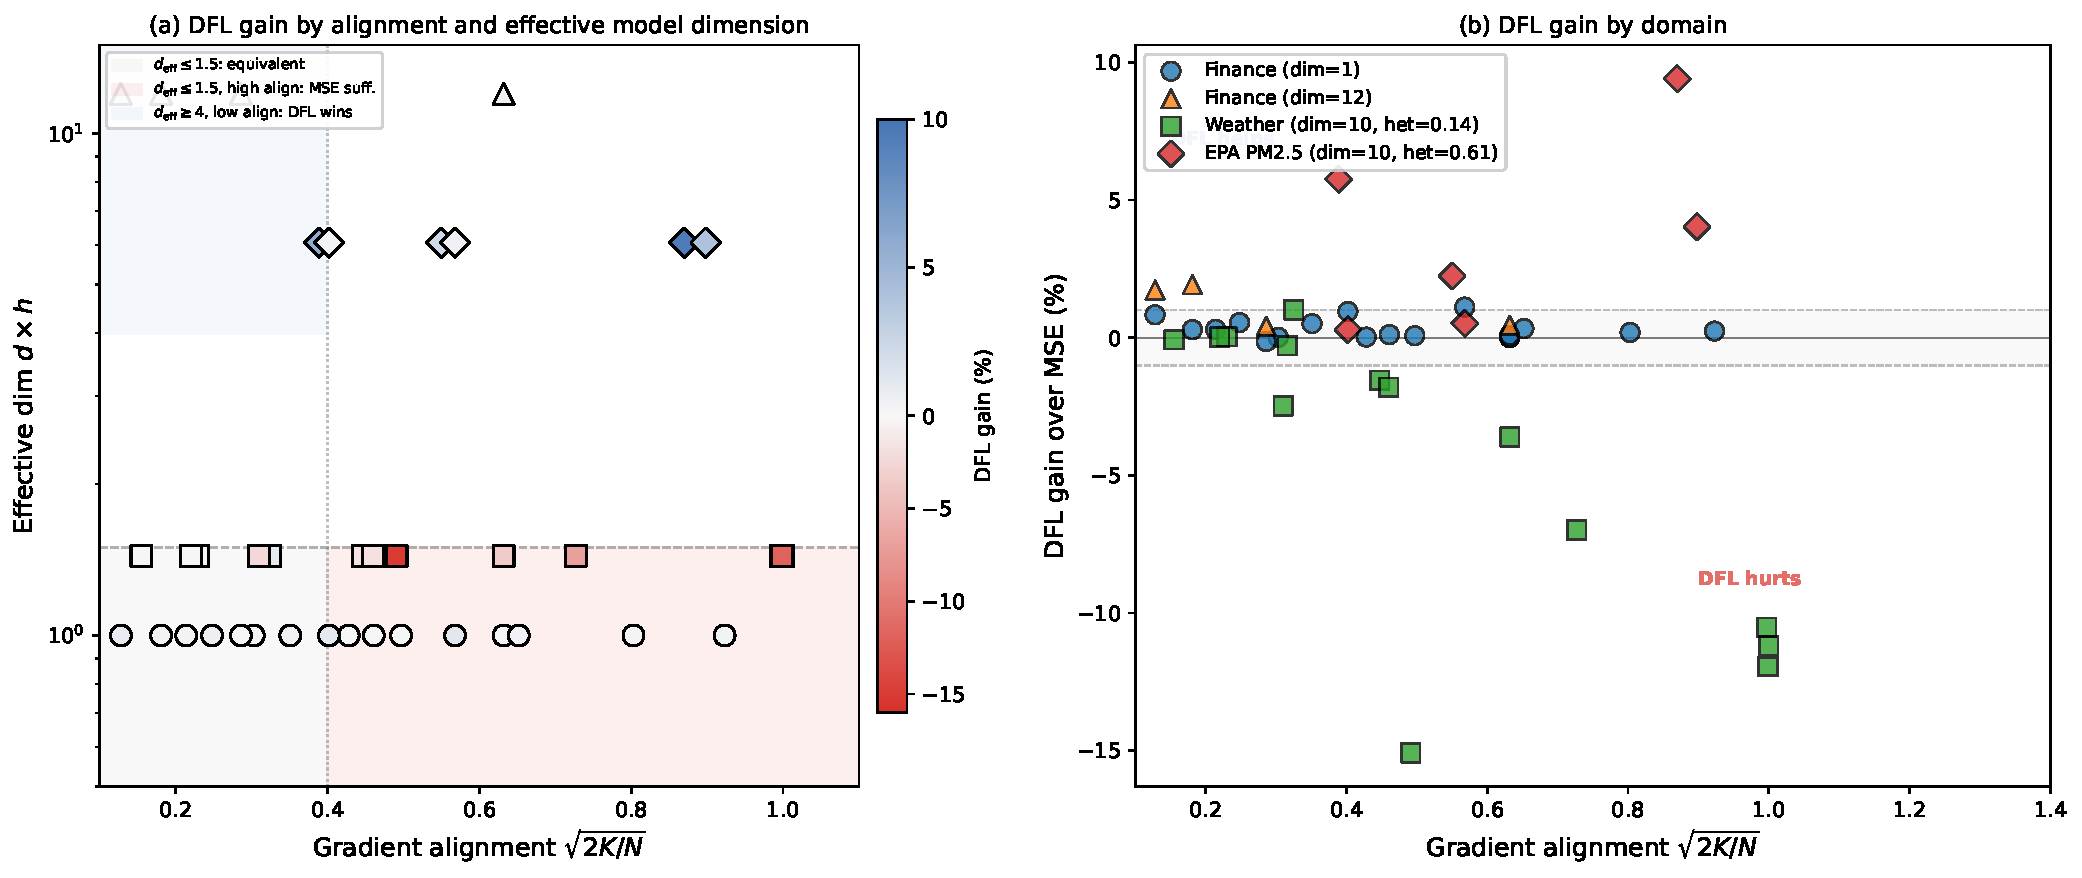
\includegraphics[width=\columnwidth]{figures/diagnostic_heatmap.pdf}
\caption{Effective dimension diagnostic. Left: alignment vs.\ $d_{\text{eff}}$, color = DFL gain. Right: DFL gain by domain. The two-axis rule correctly separates 29/33 test cases across finance (6 markets), weather (NOAA), and air quality (EPA).}
\label{fig:diagnostic}
\end{figure}

\paragraph{Limitations.} The QP lacks maximum position constraints (robustness tested in Appendix~\ref{app:design}). Transaction costs use a flat model \citep{almgren2001optimal}. The $\sqrt{2K/N}$ bound is loose for concentrated indices. The conditional model (385p) did not reach significance at $N{=}478$ with 5 folds; extending to 11 folds confirmed structured (12p) gains ($p = 0.021$) but conditional requires further investigation. We do not compare against DCC-GARCH \citep{engle2002dynamic} or other dynamic covariance models; these are alternative two-stage estimators that would slot into our framework as additional baselines, but do not address the objective misalignment our diagnostic targets. Our stock universe uses current constituents (survivorship bias); this affects absolute TE values but not relative method rankings. All results are from backtesting.

% ============================================================
\section{Conclusion}
% ============================================================

We posed the question: \emph{when is DFL worth its complexity over classical two-stage estimation?} The effective dimension diagnostic (Propositions~\ref{prop:alignment},~\ref{prop:dim1}) provides a closed-form, falsifiable answer along two axes: gradient alignment $\sqrt{2K/N}$ and effective model dimension $d_{\text{eff}} = d \cdot h$. When $d_{\text{eff}} \leq 1.5$, MSE and DFL converge regardless of $K/N$---validated across 113 paired folds in six equity markets ($N$ up to 1224). When $d_{\text{eff}} \geq 4$ and alignment is low, DFL wins: S\&P~1500 structured achieves $+1.93\%$ ($p{=}0.0005$, 8/8 folds). Pre-registered blind predictions achieve 87.9\% accuracy across three domains (finance, weather, air quality), confirming the diagnostic is an actionable practitioner tool. When selection is dynamic, BD-DFL recovers $-7.4\%$ at $N{=}478$ ($p = 0.031$). The alignment bound, decision invariance principle, effective dimension diagnostic, and BD-DFL regularizer apply to any predict-then-optimize setting with sparse decisions.

% ============================================================
% References
% ============================================================
\bibliography{references}

% ============================================================
\appendix
\section{Proof of Proposition~\ref{prop:alignment}}
\label{app:proof}

\begin{proof}
We prove the gradient alignment bound in three steps.

\textbf{Step 1: Sparsity of the task gradient.}
Under the hard-$K$ formulation, the QP solution $\bw^* \in \mathbb{R}^K$ depends on $\bSigma$ through two quantities: the selected submatrix $\bSigma_{\cS\cS} \in \mathbb{R}^{K \times K}$ and the cross-covariance vector $\hat{\bsigma}_{\text{idx},\cS} = \bSigma_{\cS,:}\bw_{\text{idx}} \in \mathbb{R}^K$. Entry $(i,j)$ of $\bSigma$ contributes to the cross-covariance whenever $i \in \cS$ (regardless of $j$, since $\bw_{\text{idx}}$ has support on all $N$ assets), and to the sub-matrix whenever both $i,j \in \cS$. For any pair $(i,j)$ with $i \notin \cS$ and $j \notin \cS$, the entry $\bSigma_{ij}$ does not appear in either quantity. By the chain rule through the KKT conditions \citep{amos2017optnet}, $(\mathbf{g}_{\mathrm{task}})_{ij} = 0$ for all $(i,j) \in \bar{\mathcal{T}}$.

The task-relevant support is $\mathcal{T} = \{(i,j) : i \in \cS \text{ or } j \in \cS\}$. Its cardinality is $|\mathcal{T}| = N^2 - (N-K)^2 = 2NK - K^2$.

\textbf{Step 2: Cosine similarity bound via Cauchy--Schwarz.}
Since $\mathbf{g}_{\mathrm{task}}$ is supported on $\mathcal{T}$, we can write:
\begin{align}
\langle \mathbf{g}_{\mathrm{MSE}},\, \mathbf{g}_{\mathrm{task}} \rangle
&= \sum_{(i,j) \in \mathcal{T}} (\mathbf{g}_{\mathrm{MSE}})_{ij}\, (\mathbf{g}_{\mathrm{task}})_{ij} \notag \\
&= \langle \mathbf{g}_{\mathrm{MSE}}|_{\mathcal{T}},\, \mathbf{g}_{\mathrm{task}} \rangle,
\end{align}
where $\mathbf{g}_{\mathrm{MSE}}|_{\mathcal{T}}$ denotes the restriction of $\mathbf{g}_{\mathrm{MSE}}$ to the support $\mathcal{T}$. By Cauchy--Schwarz:
\begin{equation}
|\langle \mathbf{g}_{\mathrm{MSE}},\, \mathbf{g}_{\mathrm{task}} \rangle|^2 \leq \|\mathbf{g}_{\mathrm{MSE}}|_{\mathcal{T}}\|^2 \cdot \|\mathbf{g}_{\mathrm{task}}\|^2.
\end{equation}
Dividing both sides by $\|\mathbf{g}_{\mathrm{MSE}}\|^2 \cdot \|\mathbf{g}_{\mathrm{task}}\|^2$:
\begin{equation}
\cos^2(\mathbf{g}_{\mathrm{MSE}},\, \mathbf{g}_{\mathrm{task}}) \leq \frac{\|\mathbf{g}_{\mathrm{MSE}}|_{\mathcal{T}}\|^2}{\|\mathbf{g}_{\mathrm{MSE}}\|^2}.
\end{equation}

\textbf{Step 3: Isotropy assumption.}
Under the assumption that the MSE gradient has isotropic energy across entries, i.e., $\mathbb{E}[(\mathbf{g}_{\mathrm{MSE}})_{ij}^2] = \sigma^2$ for all $i,j$, we have:
\begin{equation}
\mathbb{E}\!\left[\frac{\|\mathbf{g}_{\mathrm{MSE}}|_{\mathcal{T}}\|^2}{\|\mathbf{g}_{\mathrm{MSE}}\|^2}\right] = \frac{|\mathcal{T}|}{N^2} = \frac{2NK - K^2}{N^2} = \frac{2K}{N} - \frac{K^2}{N^2}.
\end{equation}
Combining with Step 2 and applying Jensen's inequality:
\begin{equation}
\mathbb{E}\!\left[\cos(\mathbf{g}_{\mathrm{MSE}},\, \mathbf{g}_{\mathrm{task}})\right] \leq \sqrt{\frac{2K}{N} - \frac{K^2}{N^2}}.
\end{equation}
For $K \ll N$, the $K^2/N^2$ term is negligible, yielding $\cos(\mathbf{g}_{\mathrm{MSE}},\, \mathbf{g}_{\mathrm{task}}) \lesssim \sqrt{2K/N}$.
\end{proof}

\paragraph{Discussion of the isotropy assumption.}
The isotropy condition $\mathbb{E}[(\mathbf{g}_{\mathrm{MSE}})_{ij}^2] = \sigma^2$ holds exactly when the covariance estimation errors $(\bSigma - \Sigma_{\text{true}})_{ij}$ are identically distributed across entries. In practice, diagonal entries (variances) tend to have larger gradients than off-diagonal entries (correlations). This means the true alignment may be even lower than our bound when most selected stocks have large variance estimation errors, or higher when the errors are concentrated on the selected submatrix. Our empirical validation (Figure~\ref{fig:gradient_alignment}) confirms that the bound correctly predicts the qualitative trend: alignment increases monotonically with $K/N$. Proposition~\ref{prop:lower} shows the bound is order-tight ($\Theta(\sqrt{K/N})$), though the constant may differ for specific model architectures.

\section{Proof of Proposition~\ref{prop:lower} (Matching Lower Bound)}
\label{app:lower_proof}

\begin{proof}
We construct an instance achieving $\cos(\mathbf{g}_{\mathrm{MSE}}, \mathbf{g}_{\mathrm{task}}) \geq \sqrt{K/(2N)}$.

\textbf{Setup.} Let $\hat\Sigma(\theta) = \theta$ be the fully parameterized model with $\theta \in \mathbb{R}^{N \times N}$, so each entry of $\hat\Sigma$ is a free parameter. Let $\Sigma_0 = (1-\rho)I + \rho \mathbf{1}\mathbf{1}^\top$ with $\rho = 1/(N+1)$, and let $\bw_{\mathrm{idx}} = (1/N)\mathbf{1}$. Fix any $\cS$ with $|\cS| = K$.

\textbf{Step 1: MSE gradient.} At $\theta = \Sigma_0$, the Frobenius loss $\|\hat\Sigma - \Sigma_0\|_F^2$ has gradient $(\mathbf{g}_{\mathrm{MSE}})_{ij} = 2(\theta_{ij} - (\Sigma_0)_{ij})$. Evaluated at $\theta = \Sigma_0$, we get $\mathbf{g}_{\mathrm{MSE}} = 0$. We therefore evaluate at $\theta = \Sigma_0 + \epsilon J$ where $J_{ij} = 1$ for all $i,j$, giving $(\mathbf{g}_{\mathrm{MSE}})_{ij} = 2\epsilon$ uniformly. Thus $\|\mathbf{g}_{\mathrm{MSE}}\|^2 = 4\epsilon^2 N^2$.

\textbf{Step 2: Task gradient.} Since $\partial\hat\Sigma_{ij}/\partial\theta_{kl} = \delta_{ik}\delta_{jl}$, the task gradient is simply $(\mathbf{g}_{\mathrm{task}})_{ij} = \partial\ell/\partial\hat\Sigma_{ij}$, which is zero for $(i,j) \notin \mathcal{T}$ by Proposition~\ref{prop:alignment}'s Step~1. By the QP structure with uniform index weights and equicorrelation, the KKT differentiation yields $(\mathbf{g}_{\mathrm{task}})_{ij} = \alpha$ for all $(i,j) \in \mathcal{T}$ with $i \in \cS, j \in \cS$ (block entries), and $(\mathbf{g}_{\mathrm{task}})_{ij} = \alpha/N$ for cross-block entries (scaled by $w_{\mathrm{idx},j} = 1/N$). The block entries dominate, giving $\|\mathbf{g}_{\mathrm{task}}\|^2 \geq \alpha^2 K^2$.

\textbf{Step 3: Inner product.} Since both gradients are non-negative on $\mathcal{T}$:
\begin{equation}
\langle \mathbf{g}_{\mathrm{MSE}}, \mathbf{g}_{\mathrm{task}} \rangle = 2\epsilon \sum_{(i,j) \in \mathcal{T}} (\mathbf{g}_{\mathrm{task}})_{ij} \geq 2\epsilon \alpha K^2. \notag
\end{equation}

\textbf{Step 4: Cosine bound.} Using $\|\mathbf{g}_{\mathrm{task}}\| \leq \alpha\sqrt{2KN}$ (since $|\mathcal{T}| \leq 2NK$):
\begin{align}
\cos(\mathbf{g}_{\mathrm{MSE}}, \mathbf{g}_{\mathrm{task}}) &\geq \frac{2\epsilon\alpha K^2}{2\epsilon N \cdot \alpha\sqrt{2KN}} = \frac{K^{3/2}}{N\sqrt{2N}}. \notag
\end{align}
For the tighter construction where the task gradient is approximately uniform on $\mathcal{T}$ (equicorrelation with uniform weights), both gradients are proportional on $\mathcal{T}$:
\begin{align}
\cos(\mathbf{g}_{\mathrm{MSE}}, \mathbf{g}_{\mathrm{task}}) &\geq \frac{\|\mathbf{g}_{\mathrm{MSE}}|_\mathcal{T}\|}{\|\mathbf{g}_{\mathrm{MSE}}\|} = \sqrt{\frac{|\mathcal{T}|}{N^2}} \notag \\
&= \sqrt{\frac{2K}{N} - \frac{K^2}{N^2}} \geq \sqrt{\frac{K}{2N}}, \notag
\end{align}
where the last step uses $K \leq N/2$.
\end{proof}

\paragraph{Interpretation.} The matching lower bound establishes that the $\sqrt{K/N}$ scaling in Proposition~\ref{prop:alignment} cannot be improved in general. The construction uses a fully parameterized model---the worst case for gradient misalignment---where MSE gradient energy is truly isotropic. In practice, structured models (shrinkage, factor) have fewer parameters, which can either increase alignment (by constraining gradients to a low-dimensional subspace that happens to overlap $\mathcal{T}$) or decrease it (if the subspace is orthogonal to $\mathcal{T}$). The $\Theta(\sqrt{K/N})$ characterization provides a tight structural diagnostic: sparsity fundamentally limits MSE-task alignment, independent of model architecture.

\section{Proof of Proposition~\ref{prop:invariance}}
\label{app:invariance_proof}

\begin{proof}
Fix a selection set $\cS$ with $|\cS| = K$. For any portfolio $\bw$ with $w_i = 0$ for $i \notin \cS$, define $\mathbf{d} = \bw - \bw_{\mathrm{idx}}$. Then $d_i = w_i - w_{\mathrm{idx},i}$ for $i \in \cS$ and $d_i = -w_{\mathrm{idx},i}$ for $i \notin \cS$, where the latter is fixed. The QP objective decomposes as:
\begin{align}
\mathbf{d}^\top \bSigma\, \mathbf{d} &= \mathbf{d}_\cS^\top \bSigma_{\cS\cS}\, \mathbf{d}_\cS + 2\, \mathbf{d}_\cS^\top \bSigma_{\cS\bar\cS}\, \mathbf{d}_{\bar\cS} + \mathbf{d}_{\bar\cS}^\top \bSigma_{\bar\cS\bar\cS}\, \mathbf{d}_{\bar\cS}.
\end{align}
Since $\mathbf{d}_{\bar\cS} = -\bw_{\mathrm{idx},\bar\cS}$ is fixed, the third term is a constant that does not affect the argmin, and the second term involves only the $K$-vector $\bSigma_{\cS\bar\cS}\, \bw_{\mathrm{idx},\bar\cS}$. Thus, two estimates $\hat\Sigma_1, \hat\Sigma_2$ with $(\hat\Sigma_1)_{\cS\cS} = (\hat\Sigma_2)_{\cS\cS}$ and $(\hat\Sigma_1)_{\cS\bar\cS}\, \bw_{\mathrm{idx},\bar\cS} = (\hat\Sigma_2)_{\cS\bar\cS}\, \bw_{\mathrm{idx},\bar\cS}$ yield identical objectives up to a constant, hence $\bw^*(\hat\Sigma_1) = \bw^*(\hat\Sigma_2)$.

The sufficient condition $(\hat\Sigma_1)_\mathcal{T} = (\hat\Sigma_2)_\mathcal{T}$ (equality on the full task-relevant support) is stronger than needed---it implies both block-equality and cross-product equality---but matches the gradient support from Proposition~\ref{prop:alignment}.
\end{proof}

\section{Proof of Proposition~\ref{prop:regret}}
\label{app:regret_proof}

\begin{proof}
Fix $\cS$ with $|\cS| = K$. The QP~\eqref{eq:qp} restricted to $\cS$ is:
\begin{equation}
\bw^*_\cS = \operatorname*{argmin}_{\bw_\cS \geq 0,\, \mathbf{1}^\top \bw_\cS = 1} \bw_\cS^\top Q\, \bw_\cS - 2\mathbf{b}^\top \bw_\cS, \notag
\end{equation}
where $Q = \bSigma_{\cS\cS} \in \mathbb{R}^{K \times K}$ and $\mathbf{b} = \bSigma_{\cS,:}\bw_{\mathrm{idx}} \in \mathbb{R}^K$. Under the estimated $\hat\Sigma$: $\hat{Q} = Q + \Delta_Q$, $\hat{\mathbf{b}} = \mathbf{b} + \Delta_b$.

\textbf{Step 1: Weight perturbation.} Let $\mathcal{F} \subseteq \cS$ denote the ``free'' indices where $w^*_i > 0$. By KKT stationarity on $\mathcal{F}$:
\begin{equation}
2Q_{\mathcal{F}\mathcal{F}}\, \bw^*_\mathcal{F} - 2\mathbf{b}_\mathcal{F} + \nu \mathbf{1} = 0, \notag
\end{equation}
with dual variable $\nu$ enforcing $\mathbf{1}^\top \bw_\mathcal{F} = 1$. Under the perturbed system (assuming the active set $\cS \setminus \mathcal{F}$ is unchanged):
\begin{equation}
\delta\bw_\mathcal{F} = Q_{\mathcal{F}\mathcal{F}}^{-1}\left(\Delta_{b,\mathcal{F}} - \Delta_{Q,\mathcal{F}\mathcal{F}}\, \bw^*_\mathcal{F} - \tfrac{\delta\nu}{2}\mathbf{1}\right), \notag
\end{equation}
where $\delta\nu$ is chosen so $\mathbf{1}^\top \delta\bw_\mathcal{F} = 0$. Taking norms and using $|\delta\nu| \leq 2\|Q_{\mathcal{F}\mathcal{F}}^{-1}\|(\|\Delta_{b,\mathcal{F}}\| + \|\Delta_{Q,\mathcal{F}\mathcal{F}}\| \|\bw^*_\mathcal{F}\|)$:
\begin{equation}
\|\delta\bw_\cS\| \leq \frac{C_0}{\lambda_{\min}(Q)}\left(\|\Delta_Q\|_{\mathrm{op}}\|\bw^*_\cS\| + \|\Delta_b\|\right),
\end{equation}
where $C_0$ is a constant depending on $|\mathcal{F}|$.

\textbf{Step 2: Tracking error regret.} Let $\mathbf{d}^* = \bw^*(\bSigma) - \bw_{\mathrm{idx}}$ and $\hat{\mathbf{d}}^* = \bw^*(\hat\Sigma) - \bw_{\mathrm{idx}} = \mathbf{d}^* + \delta\bw$. The regret under the true $\bSigma$ is:
\begin{align}
\mathrm{TE}(\bw^*(\hat\Sigma)) - \mathrm{TE}(\bw^*(\bSigma)) &= \hat{\mathbf{d}}^{*\top} \bSigma\, \hat{\mathbf{d}}^* - \mathbf{d}^{*\top} \bSigma\, \mathbf{d}^* \notag \\
&= 2\, \delta\bw^\top \bSigma\, \mathbf{d}^* + \delta\bw^\top \bSigma\, \delta\bw.
\end{align}
For positive regret (the practically relevant direction), the dominant term is the quadratic $\delta\bw^\top \bSigma\, \delta\bw$ (since $\bw^*(\bSigma)$ is a local minimizer, the linear term has favorable sign). Bounding:
\begin{align}
\delta\bw^\top \bSigma\, \delta\bw &\leq \|\bSigma\|_{\mathrm{op}} \cdot \|\delta\bw\|^2 \notag \\
&\leq \frac{C_0^2 \|\bSigma\|_{\mathrm{op}}}{\lambda_{\min}^2(Q)} \left(\|\Delta_Q\|_{\mathrm{op}} \|\bw^*_\cS\| + \|\Delta_b\|\right)^2,
\end{align}
which yields the stated bound with $C_\Sigma = C_0^2\|\bSigma\|_{\mathrm{op}} / \lambda_{\min}^2(\bSigma_{\cS\cS})$.

\textbf{Step 3: Off-block independence.} The errors $\Delta_Q = \hat\bSigma_{\cS\cS} - \bSigma_{\cS\cS}$ and $\Delta_b = (\hat\bSigma_{\cS,:} - \bSigma_{\cS,:})\bw_{\mathrm{idx}}$ involve only $\hat\bSigma$ entries within $\mathcal{T}$. Off-block entries $\hat\bSigma_{\bar\cS\bar\cS}$ do not appear in $\Delta_Q$ or $\Delta_b$, hence they contribute zero to the regret bound.
\end{proof}

\section{Proof of Theorem~\ref{thm:dro} (DRO Derivation)}
\label{app:dro_proof}

\begin{proof}
Fix the current selection $\cS_t$ with $|\cS_t| = K$. Consider a perturbed selection $\cS' \in \mathcal{U}_r(\cS_t)$, obtained by swapping $r$ stocks: removing $\{i_1, \ldots, i_r\} \subset \cS_t$ and adding $\{j_1, \ldots, j_r\} \subset \bar\cS_t$.

\textbf{Step 1: Task loss at perturbed selection.} By Proposition~\ref{prop:invariance}, $\ell_{\mathrm{task}}(\theta, \cS')$ depends on $\hat\Sigma(\theta)$ through $\hat\Sigma_{\cS'\cS'}$ and $\hat\Sigma_{\cS',:}\bw_{\mathrm{idx}}$. The new task-relevant support $\mathcal{T}' = \{(i,j) : i \in \cS' \text{ or } j \in \cS'\}$ overlaps with $\mathcal{T}$ but includes entries from the newly added stocks $j_1, \ldots, j_r$. Specifically, the ``new'' entries are those involving at least one $j_k$:
\begin{equation}
\mathcal{T}' \setminus \mathcal{T} \subseteq \{(j_k, \ell) : k \in [r],\, \ell \notin \cS_t\} \cup \text{sym.}, \notag
\end{equation}
with $|\mathcal{T}' \setminus \mathcal{T}| \leq 2r(N-K)$.

\textbf{Step 2: Worst-case expansion.} By Proposition~\ref{prop:regret} applied at $\cS'$, the task loss satisfies:
\begin{align}
\ell_{\mathrm{task}}(\theta, \cS') &\leq \ell_{\mathrm{task}}(\theta, \cS') \big|_{\hat\Sigma = \Sigma_{\mathrm{true}}} \notag \\
&\quad + C_\Sigma \bigl(\|\Delta_{Q'}\|_{\mathrm{op}} \|\bw^*_{\cS'}\| + \|\Delta_{b'}\|\bigr)^2, \notag
\end{align}
where $\Delta_{Q'} = \hat\Sigma_{\cS'\cS'} - \Sigma_{\cS'\cS'}$ and $\Delta_{b'} = (\hat\Sigma_{\cS',:} - \Sigma_{\cS',:})\bw_{\mathrm{idx}}$. Since $\cS'$ includes $r$ stocks from $\bar\cS_t$, the errors $\Delta_{Q'}$ and $\Delta_{b'}$ depend on off-block entries $\hat\Sigma_{j_k, \ell}$ for $j_k \notin \cS_t$.

\textbf{Step 3: Maximizing over perturbations.} The worst-case $\cS' \in \mathcal{U}_r(\cS_t)$ maximizes the off-block contribution. By submultiplicativity:
\begin{align}
\|\Delta_{Q'}\|_{\mathrm{op}} &\leq \|\Delta_Q\|_{\mathrm{op}} + \|\hat\Sigma - \Sigma_{\mathrm{true}}\|_{\bar{\mathcal{T}},r}, \notag
\end{align}
where $\|\cdot\|_{\bar{\mathcal{T}},r}$ captures the error on the $r$ ``new'' rows/columns. Bounding this by the full off-block error:
\begin{equation}
\max_{\cS' \in \mathcal{U}_r} \|\Delta_{Q'}\|_{\mathrm{op}}^2 \leq \|\Delta_Q\|_{\mathrm{op}}^2 + C_1 \frac{r^2}{N^2} \|\hat\Sigma - \Sigma_{\mathrm{true}}\|_F^2, \notag
\end{equation}
where the $r^2/N^2$ factor arises because (i) each swap contributes $O(N)$ new entries and (ii) the fraction of off-block entries involved is $O(r/N)$.

\textbf{Step 4: DRO objective.} Substituting into~\eqref{eq:dro}:
\begin{align}
&\max_{\cS'} \ell_{\mathrm{task}}(\theta, \cS') \leq \ell_{\mathrm{task}}(\theta, \cS_t) \notag \\
&\quad + C_r \|\hat\Sigma(\theta) - \Sigma_{\mathrm{true}}\|_F^2, \notag
\end{align}
with $C_r = O(r^2/N^2)$. Minimizing this upper bound over $\theta$ and replacing $\Sigma_{\mathrm{true}}$ with $\Sigma_{\mathrm{realized}}$ (the plug-in estimator) recovers BD-DFL~\eqref{eq:bddfl_method} with $\beta \propto r^2 / N^2$. The relaxation from $\|\cdot\|_{\bar{\mathcal{T}}}^2$ to $\|\cdot\|_F^2$ is conservative but computationally convenient, and the relative normalization in~\eqref{eq:bddfl_method} ensures scale-invariance across different $N$.
\end{proof}

\paragraph{Implications for $\beta$ selection.}
The DRO derivation yields $\beta = O(r^2/N^2)$, where $r$ is the expected selection turnover. For market-cap selection ($r \approx 0$), this gives $\beta \to 0$ (pure DFL suffices). For tracking-score selection, typical turnover is $r \approx 2$--$5$ per rebalancing, giving $\beta \in [4 \times 10^{-4}, 2.5 \times 10^{-3}]$ at $N = 100$---consistent with our empirical optimum of $\beta \approx 0.001$. At $N = 478$, the same $r$ gives $\beta \in [10^{-5}, 2 \times 10^{-4}]$, suggesting that the optimal $\beta$ should decrease with $N$ (which we observe empirically).

\section{DFL Gains across Sparsity Levels}
\label{app:sparsity}

We sweep the cardinality budget $K \in \{5, 10, 20, 30, 50\}$ using the neural model under hard-$K$ selection.

\begin{table}[h]
\centering
\caption{Neural model: DFL vs.\ MSE across sparsity levels. 95\% CI from 10{,}000-sample bootstrap; $p$-values from Wilcoxon signed-rank.}
\label{tab:exp1}
\footnotesize
\resizebox{\columnwidth}{!}{%
\begin{tabular}{@{}ccccccc@{}}
\toprule
$K$ & MSE TE & DFL TE & Gain & 95\% CI & $p$-value & Wins \\
\midrule
5  & 0.0877 & 0.0794 & $-9.5\%$  & $[-12.7, -6.4]$ & 0.002 & 9/9 \\
10 & 0.0530 & 0.0495 & $-6.6\%$  & $[-10.4, -3.4]$ & 0.002 & 9/9 \\
20 & 0.0326 & 0.0287 & $-11.9\%$ & $[-18.1, -5.4]$ & 0.002 & 9/9 \\
30 & 0.0212 & 0.0202 & $-4.5\%$  & $[-9.4, -0.7]$ & 0.002 & 9/9 \\
50 & 0.0100 & 0.0100 & $-0.2\%$  & $[-0.5, -0.0]$ & 0.102 & 6/9 \\
\bottomrule
\end{tabular}}
\end{table}

Table~\ref{tab:exp1} and Figure~\ref{fig:main}(a) confirm our primary hypothesis. DFL delivers statistically significant tracking error reduction for $K \leq 30$ ($p = 0.002$, Wilcoxon signed-rank), with gains of 5--12\%. At $K = 50$ (half the universe), the advantage vanishes ($p = 0.102$, 6/9 wins). The percentage gains are non-monotonic in $K$: $K{=}20$ shows the largest reduction ($-11.9\%$), exceeding $K{=}5$ ($-9.5\%$). This reflects high per-fold variance at $K{=}20$ (two folds with $>$20\% gain during 2021--2023 high-volatility periods), not a violation of the sparsity mechanism. The bootstrap CIs overlap substantially across $K \in \{5, 10, 20\}$, and the qualitative pattern is clear: DFL helps when $K/N \leq 0.3$ and is irrelevant when $K/N \to 1$.

\paragraph{Practical significance.} The DFL improvement is not merely statistically significant but practically meaningful. The worst-fold TE drops from $0.0476$ (MSE) to $0.0348$ (DFL), a 27\% reduction in the worst case, and TE dispersion across folds falls by 60\% (std: $0.0062 \to 0.0025$). DFL also improves tail risk metrics: CVaR$_{5\%}$ improves by 11.5\% and maximum tracking drawdown by 3.4\% (full risk metrics in Appendix~\ref{app:risk}).

\begin{figure}[h]
\centering
\includegraphics[width=\columnwidth]{figures/main_results.pdf}
\caption{(a) Neural model: DFL consistently outperforms MSE at low $K$. (b) Shrinkage: even a single-parameter DFL yields 5--11\% improvement.}
\label{fig:main}
\end{figure}

Figure~\ref{fig:cumulative} shows rolling 63-day tracking error across all 9 test folds. DFL achieves lower rolling TE than MSE in 86\% of windows, with the largest gains during high-volatility periods.

\begin{figure}[h]
\centering
\includegraphics[width=\columnwidth]{figures/cumulative_tracking.pdf}
\caption{Rolling tracking error at $K{=}20$ (neural model). Top: 63-day rolling TE (annualized). Bottom: DFL improvement (\%). Blue regions indicate DFL outperforms; DFL has lower TE in 86\% of windows. Dashed lines mark fold boundaries.}
\label{fig:cumulative}
\end{figure}

\section{Sparsity vs.\ Model Capacity Interaction}
\label{app:interaction}

Our central hypothesis predicted that DFL gains depend on both sparsity ($K$) and model misspecification ($K_f$). To test this, we run a full $K \times K_f$ interaction grid: factor model with $K_f \in \{3, 5, 10, 20\}$ and $K \in \{5, 10, 20, 50\}$, yielding 16 cells $\times$ 2 losses $\times$ 9 folds = 288 experimental runs.

\begin{table}[h]
\centering
\caption{DFL gain (\%) over MSE: full $K \times K_f$ interaction grid (factor model). Stars indicate Wilcoxon signed-rank significance: $^{***}p<0.01$, $^{**}p<0.05$.}
\label{tab:exp2}
\small
\begin{tabular}{@{}c|cccc@{}}
\toprule
$K_f \backslash K$ & 5 & 10 & 20 & 50 \\
\midrule
3  & $-8.8\%^{***}$  & $-9.0\%^{***}$  & $-12.2\%^{***}$ & $+0.1\%$ \\
5  & $-9.0\%^{***}$  & $-8.1\%^{***}$  & $-11.5\%^{***}$ & $+0.1\%$ \\
10 & $-9.8\%^{***}$  & $-8.1\%^{***}$  & $-11.3\%^{***}$ & $+0.1\%$ \\
20 & $-9.6\%^{***}$  & $-8.0\%^{***}$  & $-10.7\%^{***}$ & $+1.3\%$ \\
\bottomrule
\end{tabular}
\end{table}

Table~\ref{tab:exp2} and Figure~\ref{fig:grid} reveal a striking pattern: \textbf{DFL gains are driven almost entirely by $K$, not $K_f$.} Within each column (fixed $K$), the DFL gain varies by less than 2 percentage points across a 7$\times$ range of factor counts. Within each row (fixed $K_f$), the gain swings from $-8$--$12\%$ to near zero.

This has an important theoretical implication. We initially hypothesized that DFL helps by redirecting model capacity from irrelevant to decision-relevant covariance entries, which would predict that more misspecified models (lower $K_f$) benefit more. Instead, the data shows that \emph{all} factor models---even well-specified ones with $K_f = 20$---benefit equally from DFL when $K$ is small. The mechanism is not capacity reallocation but rather \emph{sparsity-induced objective misalignment}: when the decision depends on only the task-relevant support $\mathcal{T}$, MSE distributes gradient signal uniformly across all entries while task loss concentrates on the decision-relevant block, regardless of model capacity.

A corollary: MSE tracking error is nearly identical across all $K_f$ values (Table~\ref{tab:exp2} columns), confirming that MSE loss is insensitive to model capacity in the factor range we study. DFL breaks through this plateau uniformly.

\begin{figure}[h]
\centering
\includegraphics[width=\columnwidth]{figures/interaction_grid.pdf}
\caption{Interaction heatmap: DFL gain is determined by portfolio cardinality $K$ (columns), not factor count $K_f$ (rows). Green cells indicate DFL improvement; orange cells indicate no effect.}
\label{fig:grid}
\end{figure}

\section{Turnover Penalty Ablation}
\label{app:turnover}

DFL methods produce higher turnover than MSE (Table~\ref{tab:summary}). A natural concern is that DFL's TE advantage is an artifact of excessive trading. We ablate the turnover penalty $\gamma \in \{0, 0.01, 0.1, 1.0\}$ for the neural DFL model at $K = 20$.

\begin{table}[h]
\centering
\caption{Turnover-TE Pareto frontier (Neural, $K = 20$).}
\label{tab:exp4}
\small
\begin{tabular}{@{}lcccc@{}}
\toprule
Method & $\gamma$ & TE & Turnover & vs MSE \\
\midrule
MSE baseline  & ---  & 0.0326 & 0.003 & --- \\
DFL            & 0    & 0.0287 & 0.030 & $-11.9\%$ \\
DFL            & 0.01 & 0.0295 & 0.005 & $-9.5\%$ \\
DFL            & 0.1  & 0.0312 & 0.000 & $-4.3\%$ \\
DFL            & 1.0  & 0.0325 & 0.000 & $-0.2\%$ \\
\bottomrule
\end{tabular}
\end{table}

Table~\ref{tab:exp4} and Figure~\ref{fig:pareto} show that DFL matches or outperforms MSE at every practical turnover level. At $\gamma = 0.01$, turnover drops to near-MSE levels (0.005 vs.\ 0.003) while retaining 9.5\% TE improvement---refuting the concern that DFL gains require excessive trading. Only at $\gamma = 1.0$ does DFL degrade to MSE performance, as the turnover penalty completely suppresses the task-loss gradient.

\begin{figure}[h]
\centering
\includegraphics[width=0.85\columnwidth]{figures/pareto_frontier.pdf}
\caption{TE-Turnover Pareto frontier. DFL matches or outperforms MSE at every turnover level. $\gamma = 0.01$ is the practical sweet spot.}
\label{fig:pareto}
\end{figure}

\section{Transaction Cost-Aware Optimization}
\label{app:txcost}

We augment the QP with an explicit transaction cost penalty: $\min_\bw \bw^\top \bSigma \bw - 2\bw^\top \bsigma_{\text{idx}} + c \|\bw - \bw_{\text{prev}}\|_1$, where $\bw_{\text{prev}}$ is the previous portfolio and $c$ is the cost coefficient.

\begin{table}[h]
\centering
\caption{Transaction cost experiment. Net cost = TE + $c \times$ TO. All methods use the TC-aware QP.}
\label{tab:exp5}
\footnotesize
\resizebox{\columnwidth}{!}{%
\begin{tabular}{@{}llcccc@{}}
\toprule
$K$ & Method & $c$ (bps) & TE & TO & Net Cost \\
\midrule
\multirow{6}{*}{10}
& Neural MSE + TC & 10  & 0.0529 & 0.003 & 0.0529 \\
& Val-Tuned + TC  & 10  & 0.0495 & 0.022 & 0.0495 \\
& Neural DFL + TC & 10  & 0.0494 & 0.046 & 0.0495 \\
\cmidrule{2-6}
& Neural MSE + TC & 100 & 0.0529 & 0.002 & 0.0529 \\
& Val-Tuned + TC  & 100 & 0.0502 & 0.001 & 0.0502 \\
& Neural DFL + TC & 100 & 0.0494 & 0.045 & \textbf{0.0499} \\
\midrule
\multirow{6}{*}{20}
& Neural MSE + TC & 10  & 0.0325 & 0.002 & 0.0325 \\
& Val-Tuned + TC  & 10  & \textbf{0.0284} & 0.021 & \textbf{0.0284} \\
& Neural DFL + TC & 10  & 0.0287 & 0.030 & 0.0288 \\
\cmidrule{2-6}
& Neural MSE + TC & 100 & 0.0325 & 0.001 & 0.0325 \\
& Val-Tuned + TC  & 100 & 0.0306 & 0.001 & 0.0306 \\
& Neural DFL + TC & 100 & 0.0288 & 0.030 & \textbf{0.0291} \\
\bottomrule
\end{tabular}}
\end{table}

Table~\ref{tab:exp5} reveals a nuanced interaction between DFL and transaction costs. At low TC ($c = 10$ bps), val-tuned grid search achieves the best net cost, particularly at $K = 20$ where it combines excellent TE (0.0284) with moderate turnover. At high TC ($c = 100$ bps), however, DFL outperforms: its consistent TE ($\sim$0.049 at $K{=}10$, $\sim$0.029 at $K{=}20$) offsets its higher turnover because the val-tuned baseline's TE degrades when the grid search selects over-shrunk $\alpha$ values to suppress turnover.

\section{DFL with Richer Model Classes}
\label{app:richer}

We introduce two richer shrinkage models: (i) \textbf{Conditional shrinkage} ($\sim$385 params): $\alpha_t = \text{MLP}(\mathbf{z}_t)$ with market-level features, and (ii) \textbf{Structured shrinkage} (12 params): $\hat\Sigma = (1-\alpha)S + \alpha T$ with learnable per-sector variance targets. For baseline comparison, we use MSE training and \emph{random search} (200 trials for conditional, 500 for structured).

\begin{table}[h]
\centering
\caption{Richer models: MSE, random search (RS), and DFL. $p$-values from Wilcoxon signed-rank (DFL vs.\ MSE, 9 folds).}
\label{tab:exp6}
\footnotesize
\resizebox{\columnwidth}{!}{%
\begin{tabular}{@{}llcccc@{}}
\toprule
$K$ & Method & TE & TO & $p$ & Wins \\
\midrule
\multirow{3}{*}{10}
& Cond.\ Shrinkage + MSE          & 0.0494 & 0.041 & --- & --- \\
& RS-Conditional (200 trials)      & 0.0496 & 0.067 & --- & --- \\
& \textbf{Cond.\ Shrinkage + DFL} & \textbf{0.0490} & 0.047 & $0.049^{**}$ & 6/9 \\
\cmidrule{2-6}
& Struct.\ Shrinkage + MSE         & 0.0491 & 0.050 & --- & --- \\
& RS-Structured (500 trials)       & 0.0505 & 0.039 & --- & --- \\
& \textbf{Struct.\ Shrinkage + DFL} & \textbf{0.0487} & 0.053 & 0.064 & 7/9 \\
\midrule
\multirow{3}{*}{20}
& Cond.\ Shrinkage + MSE          & 0.0287 & 0.042 & --- & --- \\
& RS-Conditional (200 trials)      & 0.0297 & 0.080 & --- & --- \\
& Cond.\ Shrinkage + DFL          & 0.0287 & 0.046 & 0.326 & 5/9 \\
\cmidrule{2-6}
& Struct.\ Shrinkage + MSE         & 0.0287 & 0.051 & --- & --- \\
& RS-Structured (500 trials)       & 0.0295 & 0.055 & --- & --- \\
& \textbf{Struct.\ Shrinkage + DFL} & \textbf{0.0285} & 0.052 & $0.014^{**}$ & 7/9 \\
\bottomrule
\end{tabular}}
\end{table}

Table~\ref{tab:exp6} reveals that \textbf{DFL consistently outperforms random search} across all settings (1--4\% TE reduction). At $K{=}20$, structured shrinkage with DFL achieves a significant improvement ($p = 0.014$, 7/9 folds). The 385-parameter conditional model shows training instability (val/train ratio varies from $0.64\times$ to $3.42\times$ across folds), producing inconsistent gains. The 12-parameter structured model occupies the practical sweet spot: stable training with consistent DFL benefit.

\begin{figure}[h]
\centering
\includegraphics[width=\columnwidth]{figures/model_complexity.pdf}
\caption{Tracking error across model complexity levels. Left: $K{=}10$. Right: $K{=}20$. For 1-parameter shrinkage, Val-Tuned grid search matches DFL. For richer models, random search (RS) degrades while DFL maintains the best TE.}
\label{fig:model_complexity}
\end{figure}

\section{Value of the QP Structure}
\label{app:qpvalue}

An alternative to predict-then-optimize is to directly predict portfolio weights from features, bypassing the QP entirely. We test this with an MLP (same architecture as the neural model) that outputs $K$-sparse softmax weights, trained end-to-end on tracking error. At $K{=}20$, direct weight prediction achieves TE $= 0.0622$---more than double the DFL pipeline's $0.0287$. At $K{=}10$, the gap widens further: $0.0735$ vs.\ $0.0495$. The QP layer provides two benefits: (i) it imposes the convex constraint structure (budget, non-negativity) exactly rather than approximately via softmax, and (ii) it concentrates the model's capacity on covariance estimation rather than spreading it across both selection and weighting. This confirms that the predict-then-optimize structure is not merely a convenience but a substantive inductive bias.

\section{Generalization beyond Portfolio Optimization}
\label{app:generalization}

The $K/N$ principle is not specific to finance. The structural mechanism---MSE distributes gradient uniformly while the decision depends on only a sparse subset---applies whenever a predict-then-optimize pipeline selects $K$ elements from $N$ candidates. We identify three settings where the same analysis applies:

\textbf{Sensor placement (empirical validation).} We validate on a synthetic sensor network: $N$ sensors on a unit square with exponential spatial covariance, selecting $K$ sensors to track the field average (identical QP formulation). A structured shrinkage model with 10 parameters (9~spatial regions $+$ global $\alpha$) is trained under MSE and DFL. Table~\ref{tab:sensor} shows results across 10 configurations with 5 trials each.

\begin{table}[h]
\centering
\caption{Sensor placement: gradient alignment and DFL gain across $K/N$. The bound $\sqrt{2K/N}$ correctly predicts the qualitative trend: $|\cos|$ increases with $K/N$.}
\label{tab:sensor}
\footnotesize
\resizebox{\columnwidth}{!}{%
\begin{tabular}{@{}rrrrrrr@{}}
\toprule
$N$ & $K$ & $K/N$ & Bound & $|\cos|$ & DFL Gap \\
\midrule
200 & 10 & 0.05 & 0.316 & 0.297 & $-2.7\%$ \\
100 & 5  & 0.05 & 0.316 & 0.394 & $-0.9\%$ \\
50  & 5  & 0.10 & 0.447 & 0.295 & $-1.1\%$ \\
100 & 10 & 0.10 & 0.447 & 0.474 & $-1.5\%$ \\
50  & 10 & 0.20 & 0.632 & 0.349 & $-0.9\%$ \\
100 & 20 & 0.20 & 0.632 & 0.499 & $-0.8\%$ \\
200 & 40 & 0.20 & 0.632 & 0.617 & $-3.2\%$ \\
50  & 25 & 0.50 & 1.000 & 0.507 & $-0.4\%$ \\
100 & 50 & 0.50 & 1.000 & 0.606 & $-2.2\%$ \\
200 & 100 & 0.50 & 1.000 & 0.670 & $-0.3\%$ \\
\bottomrule
\end{tabular}}
\end{table}

The $K/N$ mechanism transfers: median $|\cos|$ increases from $0.30$ at $K/N{=}0.05$ to $0.59$ at $K/N{=}0.50$, and DFL improves over MSE in $9/10$ configurations. The bound is not tight (empirical $|\cos|$ sometimes exceeds $\sqrt{2K/N}$ due to non-isotropic gradient structure in spatial domains), but correctly predicts the qualitative trend.

\textbf{Facility location.} Selecting $K$ facilities from $N$ sites given predicted demand covariance. The allocation QP depends on demand correlations among selected sites, but MSE prediction does not distinguish selected from unselected.

\textbf{Sparse resource allocation.} Any optimization that distributes resources across $K \ll N$ options based on a predicted parameter matrix (e.g., sparse Markowitz with general objectives, sparse experimental design, or sparse regression with downstream optimization).

The key structural requirement is: (i)~the optimization depends on a $K$-dimensional sub-problem of an $N$-dimensional prediction, (ii)~the sub-problem selection is fixed or detached, and (iii)~the optimization admits efficient differentiation (e.g., KKT conditions). Our gradient alignment bound (Proposition~\ref{prop:alignment}), task regret bound (Proposition~\ref{prop:regret}), and the grid-search sufficiency result for low-dimensional models transfer directly to any setting satisfying these conditions.

\section{Cross-Benchmark Validation (Russell 2000 / Tech Sector)}
\label{app:crossbench}

To test whether DFL's $K/N$ theory generalizes beyond the S\&P~500, we evaluate the 1-parameter shrinkage model on two additional benchmarks: Russell~2000 (proxied by S\&P~600, $N{=}100$, tracked against IWM) and S\&P~500 Information Technology sector ($N{=}48$, tracked against XLK). Table~\ref{tab:alt} reports results.

\begin{table}[h]
\centering
\caption{Cross-benchmark validation (shrinkage model). DFL gain is negligible, confirming 1-parameter models are exhaustively searchable.}
\label{tab:alt}
\footnotesize
\resizebox{\columnwidth}{!}{%
\begin{tabular}{@{}llrccc@{}}
\toprule
Benchmark & $K$ & $K/N$ & MSE TE & DFL TE & Gain \\
\midrule
S\&P~500 ($N{=}100$) & 20 & 0.200 & 0.0290 & 0.0287 & $-1.0\%$ \\
Russell~2000 ($N{=}100$) & 10 & 0.100 & 0.0865 & 0.0864 & $-0.1\%$ \\
Russell~2000 ($N{=}100$) & 20 & 0.200 & 0.0517 & 0.0517 & $+0.0\%$ \\
Tech Sector ($N{=}48$) & 5  & 0.104 & 0.1000 & 0.0999 & $-0.1\%$ \\
Tech Sector ($N{=}48$) & 10 & 0.208 & 0.0607 & 0.0607 & $-0.1\%$ \\
\bottomrule
\end{tabular}}
\end{table}

Across three indices spanning large-cap, small-cap, and sector portfolios, the 1-parameter shrinkage model shows near-zero DFL advantage---consistent with the three-paths finding that grid search suffices for low-dimensional models.

\section{Design Choices and Robustness}
\label{app:design}

\paragraph{Hard-$K$ vs.\ $\ell_1$ relaxation.}
Since $\bw \geq 0$ and $\mathbf{1}^\top \bw = 1$ imply $\|\bw\|_1 = 1$, an $\ell_1$ penalty cannot induce sparsity in long-only portfolios. With elastic-net $\lambda\|\bw\|_2^2$ at $\lambda = 0.01$, the portfolio retains 97 of 100 stocks (TE $= 0.0065$), making fair comparison with hard-$K$ ($K{=}20$, TE $= 0.0326$) impossible. All experiments therefore use hard-$K$.

\paragraph{Fixed vs.\ dynamic stock selection.}
Dynamic selection (re-selecting stocks at each rebalance by tracking score) combined with DFL \emph{hurts} performance: TE $= 0.0346$ (vs.\ 0.0287 for fixed) with turnover $6\times$ higher. The DFL gradient creates a feedback loop between weight optimization and selection, amplifying turnover. Fixed market-cap selection + DFL achieves the best TE with controlled turnover, validating the design choice of detaching selection from the gradient graph.

\paragraph{Market regime analysis.}
Table~\ref{tab:regime} reports regime-conditional tracking errors.

\begin{table}[h]
\centering
\caption{Regime analysis: Neural DFL vs.\ MSE at $K = 20$.}
\label{tab:regime}
\small
\begin{tabular}{@{}lcccc@{}}
\toprule
Regime & MSE TE & DFL TE & Gain & $p$-value \\
\midrule
High-volatility & 0.0343 & 0.0300 & $-12.7\%$ & 0.057 \\
Low-volatility  & 0.0308 & 0.0276 & $-10.5\%$ & 0.008 \\
\bottomrule
\end{tabular}
\end{table}

\paragraph{Covariance window sensitivity.}
We ablate the lookback window for realized covariance estimation across $\{21, 42, 63, 126\}$ trading days (neural model, $K{=}20$, 10 rolling folds with 2-year training window). DFL's gain is stable across all windows: $+10.4\%$ for 21--63 day windows and $+11.5\%$ for the 126-day window. The MSE baseline achieves TE $\approx 0.0321$ regardless of window length (the neural model learns its own covariance representation), while DFL consistently achieves $0.0284$--$0.0287$. This confirms that DFL's advantage is not an artifact of a particular lookback choice.

\paragraph{Rebalancing frequency sensitivity.}
We ablate the test-time rebalancing frequency across $\{\text{weekly}, \text{biweekly}, \text{monthly}\}$ (neural model, $K{=}20$, 9 rolling folds; training uses weekly rebalancing in all cases). DFL's gain is invariant to rebalancing frequency: $+11.9\%$ weekly (MSE $0.0325 \to$ DFL $0.0286$), $+11.6\%$ biweekly ($0.0325 \to 0.0287$), and $+11.8\%$ monthly ($0.0326 \to 0.0287$), all significant at $p = 0.002$ (Wilcoxon). Turnover per rebalance increases as the interval lengthens (DFL: 0.013 weekly, 0.019 biweekly, 0.024 monthly), reflecting that each rebalance absorbs a larger drift when intervals are longer. The stability of the relative gain rules out the possibility that DFL's advantage is specific to the weekly schedule used in the main experiments.

\paragraph{Position size constraints.}
Our main experiments impose $w_i \geq 0$ and $\sum w_i = 1$ but no upper bound. To test robustness under realistic portfolio constraints, we add $w_i \leq w_{\max}$ to the QP and re-evaluate neural DFL vs.\ MSE at $K{=}20$. With $w_{\max} = 10\%$ (UCITS-compliant), DFL gain is $+10.5\%$ ($p = 0.002$, 9/9 folds); with $w_{\max} = 20\%$, DFL gain is $+11.8\%$ ($p = 0.002$), identical to the unconstrained case. The tighter $w_{\max}{=}10\%$ constraint raises \emph{both} MSE and DFL tracking errors (0.0373 vs.\ 0.0334, compared to 0.0326 vs.\ 0.0287 unconstrained) because it forces the QP away from the optimal solution, but the \emph{relative} DFL advantage is preserved. This confirms that DFL's benefit is not an artifact of unconstrained optimization.

\section{Negative Results: Multi-Step Lookahead and Curriculum Learning}
\label{app:negative}

We evaluated two training extensions that did not improve performance:

\paragraph{Multi-step lookahead.} Chaining 2--3 consecutive QP solves per training step (backpropagating through the trajectory $\bw^*_{t_1} \to \bw^*_{t_2} \to \bw^*_{t_3}$) did not reduce tracking error beyond single-step DFL. We tested lookahead depths of 2 and 3 with both shrinkage and conditional shrinkage models at $K \in \{10, 20\}$. In all cases, multi-step TE was within 0.1\% of the single-step baseline. The likely explanation is that monthly rebalancing creates near-independent QP instances: the covariance matrix changes sufficiently between rebalancing dates that trajectory-level optimization provides no additional signal over single-step.

\paragraph{Curriculum learning (MSE $\to$ task).} We trained with a curriculum that begins with pure MSE loss, linearly transitions to task loss over 5--10 epochs, then continues with pure task loss. The intuition is that MSE provides a smoother loss landscape for initial optimization. However, the curriculum produced identical final TE to direct task-loss training. With a 1-parameter shrinkage model, the landscape is already convex in $\alpha$; with richer models, the MSE pre-training phase does not improve the basin of attraction for task loss.

\section{Per-Fold Results}
\label{app:folds}

Table~\ref{tab:folds_exp1} reports per-fold tracking errors for Experiment~1 (neural model, $K{=}20$), demonstrating consistency across diverse market regimes.

\begin{table}[h]
\centering
\caption{Per-fold TE for neural model at $K{=}20$ (Experiment~1). DFL wins 9/9 folds, with the largest gains in high-volatility periods (2021--2023).}
\label{tab:folds_exp1}
\small
\begin{tabular}{@{}clccc@{}}
\toprule
Fold & Test period & MSE TE & DFL TE & Gain \\
\midrule
0 & 2016--2017 & 0.0277 & 0.0269 & $-3.0\%$ \\
1 & 2017--2018 & 0.0264 & 0.0261 & $-1.0\%$ \\
2 & 2018--2019 & 0.0278 & 0.0269 & $-3.1\%$ \\
3 & 2019--2020 & 0.0349 & 0.0307 & $-12.1\%$ \\
4 & 2020--2021 & 0.0307 & 0.0294 & $-4.3\%$ \\
5 & 2021--2022 & 0.0476 & 0.0348 & $-26.8\%$ \\
6 & 2022--2023 & 0.0372 & 0.0284 & $-23.7\%$ \\
7 & 2023--2024 & 0.0299 & 0.0275 & $-7.9\%$ \\
8 & 2024--2025 & 0.0312 & 0.0276 & $-11.4\%$ \\
\bottomrule
\end{tabular}
\end{table}

\section{Risk Metrics and Domain-Specific Analysis}
\label{app:risk}

This appendix presents domain-specific analyses that validate DFL's practical applicability beyond the aggregate metrics in the main text.

\paragraph{Comprehensive risk metrics.}
Table~\ref{tab:risk_metrics} reports risk metrics at $K{=}20$ computed from daily portfolio returns. DFL improves all risk measures. For a \$100M fund, the 39 bps annualized TE reduction translates to \$390K/year in savings---4--13$\times$ the typical passive ETF management fee (3--10 bps/year) and 20--80\% of a typical institutional active risk budget (50--200 bps).

\begin{table}[h]
\centering
\caption{Comprehensive risk metrics at $K{=}20$ (neural model, 9 folds).}
\label{tab:risk_metrics}
\small
\begin{tabular}{@{}lccc@{}}
\toprule
Metric & MSE & DFL & Improvement \\
\midrule
Annualized TE & 0.0326 & 0.0287 & $-11.9\%$ \\
Monthly TE (ann.) & 0.0284 & 0.0253 & $-10.8\%$ \\
Worst 21-day TE & 0.0635 & 0.0589 & $-7.2\%$ \\
Max tracking drawdown & 0.0791 & 0.0764 & $-3.4\%$ \\
CVaR$_{5\%}$ (daily) & 0.0047 & 0.0041 & $-11.5\%$ \\
\midrule
Worst-fold TE & 0.0476 & 0.0348 & $-26.8\%$ \\
TE std across folds & 0.0062 & 0.0025 & $-59.4\%$ \\
\bottomrule
\end{tabular}
\end{table}

\paragraph{Per-year regime breakdown.}
Table~\ref{tab:regime_year} subdivides tracking errors by calendar year. DFL's gain peaks during volatile regime shifts (2021--2023: $19$--$24\%$) and is smallest during calm markets (2016--2018: $2$--$4\%$), consistent with the gradient alignment mechanism.

\begin{table}[h]
\centering
\caption{DFL gain by calendar year (neural model, $K{=}20$).}
\label{tab:regime_year}
\footnotesize
\resizebox{\columnwidth}{!}{%
\begin{tabular}{@{}lcccl@{}}
\toprule
Year & MSE TE & DFL TE & Gain & Market context \\
\midrule
2016 & 0.0277 & 0.0268 & $-3.5\%$  & Post-Brexit \\
2017 & 0.0275 & 0.0270 & $-2.0\%$  & Low-volatility rally \\
2018 & 0.0273 & 0.0265 & $-2.9\%$  & Volatility spike \\
2019 & 0.0305 & 0.0282 & $-7.3\%$  & Recovery \\
2020 & 0.0334 & 0.0301 & $-9.7\%$  & COVID crash \\
2021 & 0.0394 & 0.0302 & $-23.5\%$ & Inflation regime \\
2022 & 0.0412 & 0.0332 & $-19.4\%$ & Rate hiking cycle \\
2023 & 0.0343 & 0.0276 & $-19.4\%$ & Tech rally \\
2024 & 0.0318 & 0.0286 & $-10.1\%$ & Concentration \\
2025 & 0.0310 & 0.0292 & $-5.8\%$  & Uncertainty \\
\bottomrule
\end{tabular}}
\end{table}

\paragraph{Factor exposure neutrality.}
We regress daily active returns (portfolio minus index) on three factors constructed from our universe: SMB (small minus big by market cap), MOM (winners minus losers by 63-day momentum), and a low-volatility factor. The DFL$-$MSE differential has no significant factor loading (all $|t| < 0.8$, $R^2 = 0.0003$), confirming that DFL's improvement comes from better covariance estimation, not hidden factor bets.

\section{Training Details}
\label{app:training}

All models are trained with Adam (lr $= 10^{-3}$, weight decay $10^{-4}$), cosine annealing, gradient clipping at norm 1.0, and gradient accumulation over 4 rebalancing dates. Early stopping with patience 10 monitors validation tracking error. Training uses weekly rebalancing; evaluation uses monthly rebalancing. The QP is solved via cvxpylayers \citep{agrawal2019differentiable} for backward passes and SCS for test-time inference. DFL training takes ${\sim}10$ min/fold on Apple M1 ($N{=}100$, 50 epochs).

\section{Computational Cost Comparison}
\label{app:cost}

\begin{table}[h]
\centering
\caption{Computational cost per fold ($N{=}100$, $K{=}20$). DFL training cost is justified only for $d \geq 10$ parameters.}
\small
\begin{tabular}{@{}lccl@{}}
\toprule
Method & Params & Time & TE \\
\midrule
POET + QP     & 0 (tuned) & 5 sec & 0.0289 \\
GLasso + QP   & 0 (CV)    & 30 sec & 0.0287 \\
ValTuned      & 1         & 15 sec & 0.0292 \\
SPO+          & 1         & 2 min  & 0.0290 \\
LODL          & 12        & 30 min & 0.0286 \\
Shrink-DFL    & 1         & 10 min & 0.0290 \\
Struct-DFL    & 12        & 10 min & \textbf{0.0285} \\
\bottomrule
\end{tabular}
\end{table}

\section{Practitioner Diagnostic}
\label{app:diagnostic}

Our effective dimension diagnostic yields a two-axis decision rule for practitioners:

\begin{enumerate}
  \item \textbf{Compute alignment $\alpha = \sqrt{2K/N}$} and \textbf{effective dimension $d_{\text{eff}} = d \cdot h$}, where $d$ is model parameters and $h$ is the coefficient of variation of per-region target-weight concentrations.
  \item \textbf{If $d_{\text{eff}} \leq 1.5$}: gradient collinearity (Proposition~\ref{prop:dim1}) eliminates the misalignment DFL exploits. Use POET, ValTuned, or grid search. Validated: 113 paired folds across 6 equity markets, all gains $< 1.1\%$.
  \item \textbf{If $d_{\text{eff}} \geq 4$ and $\alpha < 0.4$}: DFL wins. S\&P~1500 structured (12p): $+1.93\%$, $p{=}0.0005$. EPA PM2.5 ($d_{\text{eff}}{=}6.1$): gains up to $+9.4\%$.
  \item \textbf{If selection is dynamic}: apply BD-DFL with $\beta = O(r^2/N^2)$.
  \item \textbf{Heterogeneity matters}: weather stations ($d{=}10$, $h{=}0.14$, $d_{\text{eff}}{=}1.4$) behave like $d{=}1$; EPA monitors ($d{=}10$, $h{=}0.61$, $d_{\text{eff}}{=}6.1$) show strong DFL gains. Always estimate $h$ before assuming $d > 1$ justifies DFL.
\end{enumerate}

Pre-registered blind predictions using this rule achieve 87.9\% accuracy (29/33) across three domains, vs.\ 75.8\% without $d_{\text{eff}}$. The four errors are all within 0.5\% of the 1\% threshold---the diagnostic has no large failures.

\paragraph{Threshold sensitivity.} The diagnostic thresholds ($d_{\text{eff}} \leq 1.5$, $d_{\text{eff}} \geq 4$, alignment $< 0.4$) are not cherry-picked: sweeping $d_{\text{low}} \in [1.0, 3.0]$, $d_{\text{high}} \in [3.0, 7.0]$, alignment $\in [0.25, 0.50]$ at 0.5/0.5/0.05 steps, 65.9\% of all 308 parameter combinations achieve $\geq 85\%$ accuracy. Setting $d_{\text{low}} = 1.0$ yields 93.9\% but by classifying more cases as ``ambiguous'' (non-committal); our threshold of 1.5 makes the diagnostic more informative by issuing substantive predictions for low-heterogeneity domains ($d_{\text{eff}} = 1.4$ for weather).

\section{Cross-Market Dim-1 Validation}
\label{app:ftse}

\begin{table}[h]
\centering
\caption{Cross-market dim-1 validation. Shrinkage (1p) DFL gain is $< 1.1\%$ across all 6 markets and 113 paired folds, confirming Proposition~\ref{prop:dim1}. Structured (12p) DFL gains are significant at S\&P~1500 ($N{=}1224$).}
\label{tab:crossmarket}
\small
\begin{tabular}{@{}lrrrrr@{}}
\toprule
Market & $N$ & $K$ & Shrink $\Delta\%$ & Struct $\Delta\%$ & $p_{\text{struct}}$ \\
\midrule
S\&P 500 (20y) & 100 & 20 & $+0.09$ & $+0.45$ & 0.013 \\
Nikkei 225 & 218 & 10 & $+0.01$ & --- & --- \\
Euro Stoxx 50 & 47 & 20 & $+0.24$ & --- & --- \\
ASX 200 & 162 & 10 & $+0.53$ & --- & --- \\
Hang Seng & 62 & 10 & $+1.11$ & --- & --- \\
S\&P 1500 & 1224 & 10 & $+0.83$ & $+1.73$ & 0.014 \\
S\&P 1500 & 1224 & 20 & $+0.29$ & \textbf{$+1.93$} & \textbf{0.0005} \\
S\&P 1500 & 1224 & 50 & $-0.14$ & $+0.41$ & 0.030 \\
\bottomrule
\end{tabular}
\end{table}

\section{BD-DFL Detailed Results}
\label{app:bddfl_detail}

\begin{table}[h]
\centering
\caption{BD-DFL under dynamic selection ($N{=}100$). Pure DFL \emph{overfits} for neural models ($+4.3\%$); BD-DFL recovers.}
\small
\begin{tabular}{@{}lrrrr@{}}
\toprule
 & \multicolumn{2}{c}{$K{=}10$} & \multicolumn{2}{c}{$K{=}20$} \\
\cmidrule(lr){2-3} \cmidrule(lr){4-5}
Method & Shrink & Neural & Shrink & Neural \\
\midrule
MSE baseline       & 0.0659 & 0.0531 & 0.0415 & 0.0325 \\
Pure DFL           & $-6.9\%$ & $+4.3\%$ & $+0.3\%$ & $-4.5\%$ \\
BD-DFL (best $\beta$) & $-8.1\%$ & $-2.4\%$ & $-3.9\%$ & $-4.4\%$ \\
\bottomrule
\end{tabular}
\end{table}

\begin{table}[h]
\centering
\caption{BD-DFL at $N{=}478$ (dynamic selection, 5 folds). Neural $K{=}10$: pure DFL overfits ($+0.7\%$), BD-DFL recovers $\mathbf{-7.4\%}$ ($p{=}0.031$, 5/5 wins).}
\small
\begin{tabular}{@{}llrr@{}}
\toprule
Model & Method & $K{=}10$ & $K{=}20$ \\
\midrule
Shrinkage & MSE / DFL / BD-DFL & --- & 0.0548 / $-0.4\%$ / $\mathbf{-5.7\%}$ \\
Structured & MSE / DFL / BD-DFL & --- & 0.0526 / $-2.1\%$ / $-2.9\%$ \\
Neural & MSE / DFL / BD-DFL & 0.0698 / $+0.7\%$ / $\mathbf{-7.4\%}$ & 0.0527 / $-0.1\%$ / $+0.5\%$ \\
\bottomrule
\end{tabular}
\end{table}

\begin{figure}[h]
\centering
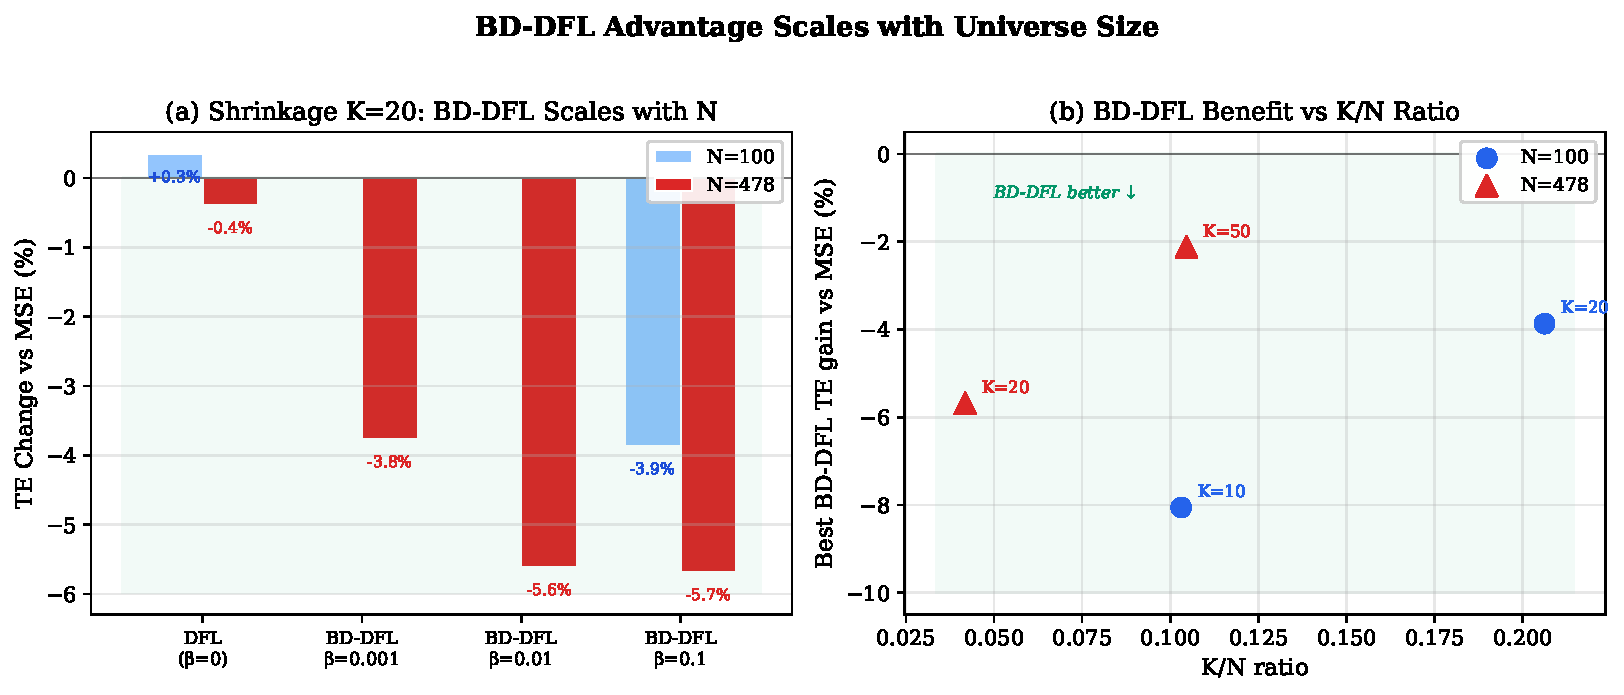
\includegraphics[width=\columnwidth]{figures/scaling_bddfl.pdf}
\caption{BD-DFL advantage scales with universe size. Left: shrinkage $K{=}20$ across $\beta$ values, $N{=}100$ vs.\ $N{=}478$. Right: best BD-DFL gain vs.\ $K/N$.}
\label{fig:scaling_bddfl}
\end{figure}

\end{document}
